\section{Introduction}\label{sec:intro}
What factors can explain the substantial and persistent increase in US household 
indebtedness over the last three decades? This question has inspired a large 
literature that has put forward several explanations. On the side of credit supply,
 the institutional framework plays a central role; \citet{CampbellHercovitz2005} 
emphasize the effects of the liberalization of the US home mortgage market in the
 early 1980s while \citet{Narajabad2012} points towards improvements in banks' 
risk assessment capabilities to explain an increase in credit lines available to 
households. On the demand side, the most influential view is arguably given by 
\citet{KruegerPerri2006} who interpret the expansion of US credit markets as the 
rational response of consumers borrowing in order to smooth out income shocks, 
the variance of which has risen over time. However, this view rests on the observed
 increase in cross-sectional income variation being largely due to a rise in the 
variance of transitory idiosyncratic shocks, an interpretation that has been called 
into question by several authors. As an example, \citet{KopczukSaezSong2010} find 
that the rise in income inequality was almost entirely driven by increases in 
permanent earnings inequality, with no mitigating effect of mobility across income
 groups that decreased at the same time as earnings inequality increased. In the
 same vein, \citet{DHPRV2013} use a confidential panel of tax returns from the 
IRS to show that all of the rise in the variance of male labour earnings between
1987 and 2009 can be attributed to a rise in the variance of the persistent part 
of income. In light of these difficulties, the present work aims to examine an 
additional mechanism that could drive household credit demand -- consumption 
habits. In this regard, this work bears some resemblance to the prominent
 \citet{Rajan2011} hypothesis that the foundations for the financial crisis of 
2007/08 were laid by a credit expansion that mostly benefited low-income 
households. This also relates to more heterodox, post-Keynesian and Marxist 
explanations of rising household indebtedness that emphasize the role of debt 
as a substitute for stagnating or declining real wages in the middle and lower
 percentiles of the income distribution (see, for example, 
\citealp{BarbaPivetti2009}), a mechanism of course that would require households
 to be -- at least for some time -- oblivious towards the realities of the path
 of their income stream. Often, behavioural explanations such as conspicuous 
consumption or household optimization based on a relative income hypothesis are 
invoked, examples include \citet{BertrandMorse2012}, who find empirical support 
for the hypothesis that consumption of lower income households is influenced by 
consumption of high income households, and \citet{vanTreeck2012}, who presents 
some calculations based on Duesenberry's (1940) relative income hypothesis. 
Here, we try to frame this argument in terms of an arguably more standard 
economic model: a life-cycle model with fully optimizing rational households 
that derive utility from current and past consumption, while facing an uncertain
 income stream that they learn about over the course of their working life. The 
basis for the present analysis is a model introduced by \citet{Guvenen2007}, in 
which the income process consists of a permanent stochastic AR(1)-component, as 
is standard in most of the literature, and an additional deterministic term,
 that is different across workers and that they have to learn about in order to
make precise forecasts of their lifetime income. This uncertainty, coupled with 
the time-inseparability of consumption introduced by habit formation, can under 
certain circumstances lead to an increase in the indebtedness even of households
 with permanently low incomes. \\
The remainder of this paper is structured as follows: Section (\ref{sec:sf}) 
presents some stylized facts on the developments of the US income and wealth 
distribution that motivate this work. Section (\ref{sec:model}) briefly lays
out the model, 
 and gives analytical results for a stripped down version of the model that 
shed light on the mechanisms through which habit formation can generate higher 
indebtedness. Section (\ref{sec:qr}) presents the results of a quantitative 
evaluation of the model using the income process parameters estimated in 
chapter \ref{ch:income}, while section (\ref{sec:calibration}) employs a 
minimum distance estimator to fit the model to the empirical distribution of 
household wealth. Section (\ref{sec:comp_stats}) performs comparative statics
on the parameters of the model to shed light on the mechanisms driving the models
success in replicating the data. Section (\ref{sec:discussion}) discusses the 
results of the chapter.

\pagebreak
\section{Stylized Facts}\label{sec:sf}
The widening inequality in the U.S. income distribution is a well documented 
feature of the data during at least the last three decades. Numerous studies 
have examined the secular rise in top incomes (\citealp{PikettySaez2003}) and 
the flattening path of middle and lower incomes (\citealp{AutorKatzKearney2005})
 and put forward explanations such as changes in relative demand and supply for 
different skill levels, the decline of union power, increases in international 
trade and competition (\citealp{Ma2013}) and the fall in the real value of the 
federal minimum wage\footnote{Some doubts on the magnitude and timing of the 
rising inequality are raised by \citet{Gordon2009}.}. While the exact timing and
 magnitude of the rise in inequality may differ slightly from one data source to 
the other and depending on the exact definition of income employed, its existence 
can be regarded as a consensus in the literature. Figure (\ref{fig:inc_ineq}) is 
taken from Attanasio, Hurst and Pistaferri (2012) and shows the evolution of 
income inequality at different points of the income distribution from 1980 to 
2010 based on PSID data. The rise in overall inequality is apparent and can be 
seen to be mostly driven by a surge in top incomes (even though, as the authors 
note, PSID data undersamples very rich households and thus most likely understates
 the rise in top incomes). 
\begin{figure}[ht]
	\centering
		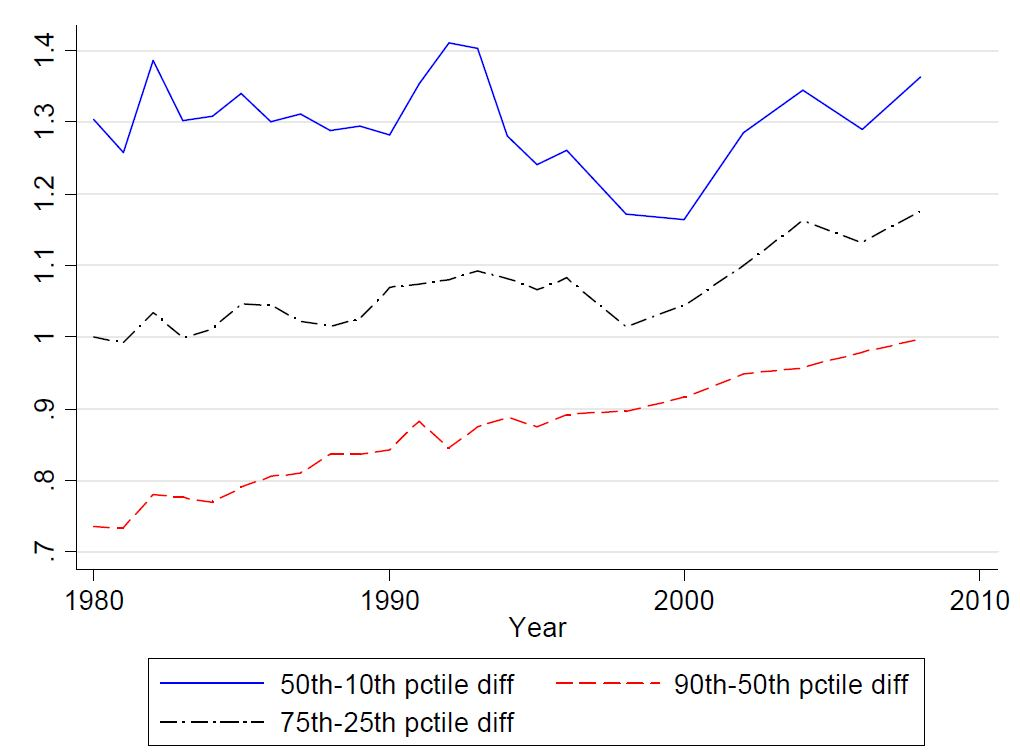
\includegraphics[width=0.85\textwidth]{inc_ineq_attanasio2012.JPG}
		\caption{Income inequality for three income differentials, 1980-2010, PSID data}
	\label{fig:inc_ineq}
\end{figure}
There exists less consensus about the evolution of consumption inequality over 
the same period. While early prominent studies such as \citet{KruegerPerri2006}
 used CEX data to argue that there has been virtually no increase in consumption 
inequality and built theoretical models that could account for this puzzle, more 
recently other authors have found a larger increase in consumption inequality 
using different data sources that arguably suffer from less measurement error than
the aggregate CEX data. \citet{HeathcotePerriViolante2010} use CEX spending data
 to document a very modest increase in consumption inequality, while 
\citet{AguiarBils2015} use the difference between income and spending in CEX data
 to document a rise in consumption inequality that is almost as large as the rise
 in income inequality and \citet{AHP2013} argue that, looking at some of the more
precisely measured items in the CEX, one finds that consumption inequality has 
indeed tracked income inequality. For the purpose of this paper, we will use 
aggregate spending data from the CEX and thus assume that consumption inequality 
has not risen to the same extent as income inequality while keeping in mind that 
this is not a foregone conclusion. We will return to this point in the last chapter. \\
Another well documented feature of the data is the rise in debt holdings of the 
private sector. As with the rise in income inequality, this development has been 
widely noted and discussed with numerous explanations put forward, including 
changes in the regulatory framework and banking technology that widened credit 
supply. Most relevant to this work is the demand side argument of \citet{KruegerPerri2006}, 
who explain the rise in indebtedness with a limited commitment model in which the
 variance of the transitory component rises and hence more insurance is required,
 and, indeed, optimal from a welfare perspective. However, as \citet{Cordoba2008}
 points out, their model produces two empirically unappealing results: for one, 
wealth holdings are not concentrated at the top of the distribution, and second, 
the model predicts a large fraction of agents in the economy with negative wealth 
holdings, when their number really is close to zero in the data. Furthermore,
 their argument is weakened by a number of studies that find changes in the 
variance of the permanent component of income shocks to be the driving force 
behind the rise in income inequality. This is hard to reconcile with the fact 
that individuals at the lower end of the income distribution are those that 
increased their debt holdings the most. Figure (\ref{fig:chg_debt_scf}) shows 
the changes in debt holdings for various debt categories calculated from SCF 
data for 1989 to 2007. 

\begin{figure}[ht]
	\centering
		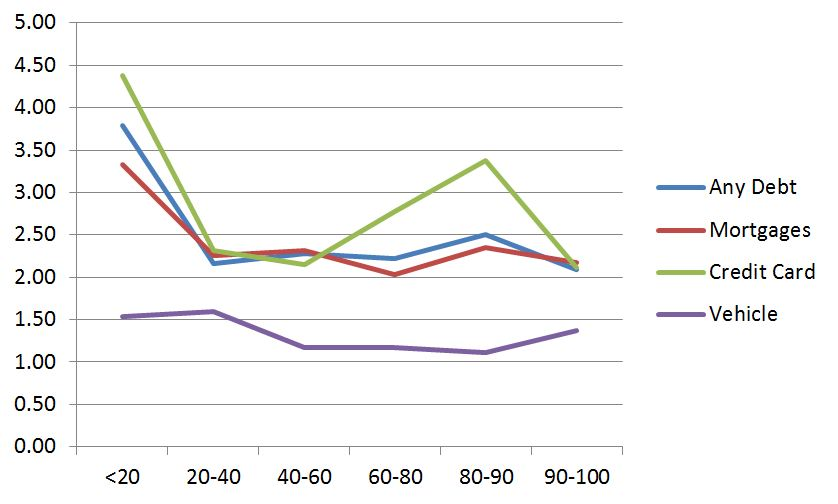
\includegraphics[width=0.85\textwidth]{chg_debt_scf}
		\caption{Changes in debt holding by income percentile, 1989-2007, Source: SCF}
	\label{fig:chg_debt_scf}
\end{figure}

While the large rise in indebtedness for the lowest income group is an artefact 
of business owners with failed businesses in the data, it is interesting to note 
that the rise in overall debt has been at least as large for the 20th to 60th 
percentile as for the highest income percentile. This comes as a surprise if one 
takes into account the higher income growth rates for individuals in higher 
income quintile since the early 1980s. Assuming that the dispersion in incomes 
is mostly driven by an increase in dispersion in the permanent component of income 
(as suggested by, among others, Kopczuk et al., 2010), a standard life-cycle model 
would suggest that while high income households should borrow against their higher 
future income, low income households wouldn't have an incentive to borrow when 
wages are stagnant. Furthermore, note that the data is not scaled by income, so 
that debt holdings relative to income have increased a lot more for lower income 
households, given that their income growth rates over the same period have been 
lower than those of higher income households. Indeed, \citet{BarbaPivetti2009} 
find that instalment loans and credit card debt amount to 59\% of disposable income 
for households in the lowest income quintile of the 2004 SCF, while they amount 
to only 11\% for the highest quintile. \\
One adjustment margin for households that could explain a decoupling of income 
and consumption inequality at least over short to medium frequencies is obviously 
saving. \citet{SaezZucman2014} find that the share of wealth holdings of the bottom 
90\% of the wealth distribution has fallen from 35\% in the mid 1980s to 23\% in 
2012, citing low growth of middle-class income, financial deregulation leading to 
predatory lending and behavioural biases in savings decisions as possible explanation. 
This paper can be seen as an attempt to investigate to what extent imperfect 
information of agents can account for the observed change in the wealth distribution.  

\begin{itemize}
\item Increase in the dispersion of wealth holdings that tracked or exceeded the 
rise in income inequality
\item Decreasing aggregate savings rate
\item Prevailing misperceptions about future economic situation (Moore 2003)
\end{itemize}

\pagebreak
\section{The Model}\label{sec:model}
The model employed is a standard incomplete markets life-cycle model of household  
consumption and savings as described in chapter \ref{ch:wealthmodels}, with the
addition of a learning mechanism for household income, as first used by 
\citet{Guvenen2007}. While this model has recently been used to study household's
portfolio choices (\citealt{ChangHongKarabarbounis2015}) and the joint evolution 
of income and consumption inequality in a rich dynamic model featuring informal
insurance mechanisms (\citealt{GuvenenSmith2014}), the implications of heterogeneous
income processes and learning for the aggregate wealth distribution have so far
not been examined to the best of our knowledge.
Consumers maximize
\begin{align}
E_0 &\left[ \sum_{t=0}^{T} \beta^{t} \frac{c_{t}^{1-\sigma}}{1-\sigma} \right] \label{eq:maxprob} \\
\intertext{s.t. } &a_{t+1} = (1+r)a_t + y_t - c_t \label{eq:bc} \\
				  &y_{t}^i = g(\theta^0, X_t^i) + f(\theta^i, X_t^i) + z_t^i + \epsilon_t^i \label{eq:incproc} \\
  				  &a_{t+1} \geq \underline{a} \label{eq:borrcons} 
\end{align}
where $c_t$ is consumption in period $t$, $a_t$ are asset holdings subject to 
a borrowing constraint  $\underline{a}$, and $y_t^i$ is individual 
income, which follows the heterogeneous income specification in logs discussed
in chapter \ref{ch:income}: 
\begin{equation*}
y_{t}^i = g(\theta^0, X_t^i) + f(\theta^i, X_t^i) + z_t^i + \epsilon_t^i 
\end{equation*}
Here, $g(\theta^0, X_t^i)$ captures age effects and individual specific 
characteristics such as education, $z_t^i$ is an autoregressive process of order
 one, and $f(\cdot)$ is an individual specific function that plays the decisive
role in introducing heterogeneity and learning in the model.
\begin{align*}
f(\theta^i, X_t^i) &= \alpha^i + \beta^i t \\
z_t^i &= \rho z_{t-1}^i + \eta_t^i \\
\theta^i &\sim N \left[ \begin{pmatrix} 0 \\ 0 \end{pmatrix}, \begin{pmatrix} \sigma_{\alpha}^2 & \sigma_{\alpha \beta} \\ \sigma_{\alpha \beta} & \sigma_{\beta}^2 \end{pmatrix} \right]
\end{align*}
The parameters $\alpha$ and $\beta$ are randomly distributed over the population 
and govern the evolution of lifetime income over time. Furthermore, they are 
unknown to individuals upon entering the labour market, meaning that in order to
 calculate an expected lifetime income to base consumption choices on, consumers 
in the model have to form beliefs over the values of their individual parameters. 
Here again we follow Guvenen in assuming that these beliefs are formed optimally
in a Bayesian fashion, which means solving a Kalman filtering problem. 
Denoting by $S^i_{t+1}$ the vector of parameters $\alpha^i$, $\beta^i$ and 
$z^i_{t+1}$ and by $F$ the coefficient vector in the state space representation,
the evolution is governed by the law of motion:
\begin{align}
\hat{S}^i_{t|t} &= \hat{S}^i_{t|t-1} + P_{t|t-1} H_t [H_t' P_{t|t-1} H_t + R]^{-1}(y_t^i - H_t' \hat{S}^i_{t|t-1}) \label{eq:KFS} \\
\hat{S}^i_{t+1|t} &= F \hat{S}^i_{t|t} \label{eq:TES}
\end{align}
where we denote by $\hat{S}^i_{t|t}$ the optimal belief about the individual specific
parameters of the income process in period $t$ after having observed the realisation
of $y_t^i$, and by $\hat{S}^i_{t+1|t}$ the optimal forecast based on those beliefs,
assuming that the transition matrix $F$ is known to the household. $P_{t|t}$ is 
the variance-covariance matrix of $\hat{S}^i_{t|t}$ and $R$  is the variance of 
the transitory shock. A similar expression can be derived for the evolution of 
$P_{t+1|t}$:
\begin{align}
P_{t|t} &= P_{t|t-1} - P_{t|t-1} H_t [ H_t' P_{t|t-1} H_t + R]^{-1} H_t' P_{t|t-1} \label{eq:KFP} \\
P_{t+1|t} &= F P_{t|t} F' + Q \label{eq:TEP}
\end{align}
With $Q$ denoting the covariance matrix of the innovation in the state space 
representation of $\hat{S}_{t+1|t}^i$ (which is basically the innovation in the 
AR(1) component of earnings). 
Given this formulation for the evolution of beliefs, we can write the recursive 
version of our maximization problem as:
\begin{equation} \label{eq:bellman}
V_t(x_t,\hat{S}^i_{t|t}) = \max_{\{c_t^i, a_{t+1}^i\}} \left\{ u(c_t) + \mathbb{E}_t \left[ V_{t+1}(x_{t+1},\hat{S}^i_{t+1|t+1}|\hat{S}^i_{t|t}) \right] \right\}
\end{equation}
which again has to be solved subject to the constraints, \ref{eq:bc}, \ref{eq:borrcons} 
and \ref{eq:KFS}-\ref{eq:TEP}. Note that given this formulation of the problem, 
all state variables appearing in the continuation value function on the right-
hand side of the Bellman equation are functions of the realisation of income 
next period, so that the expectation in \ref{eq:bellman} has to be taken only 
with respect to $\hat{y}^i_{t+1}$. The distribution of next period's expectation
of income is known exactly, conditional on current beliefs:
$$ 
\hat{y}^i_{t+1} \sim \mathcal{N}(\hat{\alpha}_{t|t} + (t+1)\hat{\beta}^i_{t|t} + \rho \hat{z}_{t|t}, \sigma^2_{\alpha} + t^2 \sigma^2_{\beta} + 2t\sigma_{\alpha \beta} + \sigma^2_{\eta} + \sigma^2_{\varepsilon}
$$
An important issue when trying to match empirical wealth distributions is the 
specification of the pension system. The household problem during retirement is 
straightforward to solve in the absence of uncertainty; it is given by
\begin{align}\label{eq:retirement}
V^R_t(a_t,\bar{y}) &= \max_{c_t, a_{t+1}} u(c_t) + \delta V^R_{t+1}(a_{t+1},y^R)
\intertext{s.t.}   &a_{t+1} = (1+r)a_t + \bar{y} - c_t \\
				   &y^R =  M(\bar{y}, \bar{Y})\\
  				   &a_{t+1} \geq \underline{a}
\end{align}
where $M$ is a benefit function that emulates the US Social Security system and 
is specified following much of the literature on life-cycle models (cp. 
\citet{STY2004}, \citet{HintermaierKoeniger2011}, \citet{GuvenenSmith2014}, 
amongst others) as a function depending on average lifetime income  of an 
individual, $\bar{y}$, relative to the economy-wide average income $\bar{Y}$:
$$
y^P = \begin{cases} 0.9\bar{y} & \text{if} \bar{y} < 0.3\bar{Y}  \\
    0.27 + 0.32(\bar{y} - 0.3) & \text{if} \bar{y} \leq 2.0\bar{Y} \\
    0.814 + 0.15(\bar{y}- 2.0) & \text{if} \bar{y} \leq 4.1\bar{Y} \\
           1.129 \bar{Y}       & \text{if} \bar{y} > 4.1 \bar{Y}
      \end{cases}
$$
Note that this system attenuates the inequality in lifetime income created by 
the stochastic process for income by providing higher replacement rates for 
poor households than for rich households. To avoid adding another state variable
to the model, we replace the true value of $\bar{y}$ by an estimate derived
from running the cross-sectional regression 
    



\subsection{Computational Algorithm}
To solve the model, we adopt a strategy similar to that in \citet{GuvenenSmith2014}.
After drawing an income distribution and simulating agent's learning given a set
of initial beliefs, we construct a three-point grid for $\hat{\alpha}$, a 
fifteen-point grid for $\hat{\beta}$ and a seven-point grid for $\hat{z}$, all
linearly spaced ranging from the lowest to the highest belief coming out of the
simulation of agent's learning process. For wealth, we choose 40 grid points, 
exponentially spaced with a higher concentration of points at low levels of wealth.
The household's pension problem can be solved analytically, while the household's 
working life problem is solved recursively on all grid points in the four-
dimensional state space. To evaluate the continuation value function on the right-
hand side of the Bellman equation, we employ quadrilinear interpolation combined
with Gauss-Hermite quadrature on ten nodes for the numerical integration
\footnote{In particular, the linear interpolation was performed using the 
\texttt{ApproXD.jl} package \citep{Oswald2014}, while the Gauss-Hermite nodes
were derived using the \texttt{FastGaussQuadrature.jl} package \citep{Townsend2015}.}. In the
simulation step, we initialise household wealth holdings by drawing from the empirical 
wealth distribution for 23 to 25 year old households from the Survey of Consumer
Finances, data that is available in \cite{HintermaierKoeniger2011}, and check 
the sensitivity of model results to this choice by comparing them to the 
alternative of zero wealth holdings at age 20 for all households. 


\pagebreak
\section{Quantitative Results}\label{sec:qr}
Given the slow learning induced by the nature of the income process, the initial 
beliefs of consumers are of crucial importance for consumption decisions in the 
first periods of live. These in turn determine a habit stock that might (depending
 on the parameter choice for $\lambda$) have a long lasting effect on the marginal 
utility of consumption in the following periods. Hence, it is important to explore
 the sensitivity of results to different initial belief vectors and think about 
reasonable parametrizations. In a more fully specified model, one could further
 introduce a trade-off for agents between "comforting" expectations about their 
own future and the cost attached to acting on overly optimistic preferences, as 
for example argued by \citet{Glaeser2004}, but such a specification would require
 the introduction of a further unknown parameter in the utility function determining
 the utility of optimistic expectations and is therefore outside the scope of 
this work. Instead, we will focus on two baseline cases and explore the 
sensitivity of results to deviations from this baseline. \\
The first case assumes that agents entering the labour market in the model at age
 25 have formed expectations based on previous observations of wage growth for 
workers in similar occupations to the one they are entering. Hence, we will assume
 that someone entering the labour market at, say, the 20th quintile of the wage 
distribution, will have expectations that were formed on the wage growth of 
workers in the 20th quintile 10 years prior to the worker entering the labour 
market. Note that this will have opposite effects on workers entering the labour
 market in the late 1970s, just before cross-sectional wage dispersion started 
to increase: while workers in low-skill occupations at the bottom of the wage 
distribution will face lower income growth rates than their predecessors, and 
thus growth rates below their expectations, workers at the high end of the wage 
distribution will see their incomes grow above expectations for the same reason. 
Thus, with this parametrization, poorer households will build up habit stocks 
that are too high relative to lifetime income early in life, with the reverse 
being true for high income households. \\
The second baseline case is inspired by the aforementioned research on people's 
inclination to hold optimistic beliefs as well as survey evidence on the 
overconfidence of economic actors. One such example would be a Gallup poll 
(\citealp{Moore2003}) in which 31\% of respondents declared to expect to be rich
 at some point in their life, a number that jumps to 51\% for the group of 18 to
 29 year olds, where \textit{rich} is defined as having an annual income of more
 than \$120,000 or assets in excess of \$1,000,000. \citet{DiPrete2007} surveys
 a number of similar polls, compares their results with PSID data and concludes 
that even accounting for subjective differences in the definition of "being rich",
 Americans significantly overestimate the opportunity for upward income mobility
 over their lifetime \footnote{Interestingly, this overconfidence seems to have 
been dampened by the financial crisis, if more recent studies are an indication.
 Compare, e.g. http://www.cnbc.com/id/44559645}. A host of similar studies can 
be found and while one can certainly question whether such obviously unreasonable 
expectations form the basis for everyday economic decisions, they do point towards
 a significant amount of unwarranted optimism about the own economic future for 
a large part of the population. With this in mind, in the second scenario the 
belief vectors are parametrized to values that exceed the realized growth rates
 for all income brackets over the entire sample period. While comparing these 
two cases already gives us a good deal of information about the sensitivity of 
results to the belief vector, in section (\ref{sec:discussion}) we will also discuss 
the results using Guvenen's (2007) parametrization to make the model results 
directly comparable and of experimenting with more extreme values of beliefs. 

\section{Calibrating the model}\label{sec:calibration}
Similar to \citet{HintermaierKoeniger2011}, we calibrate the model using a minimum 
distance estimator that minimizes the difference between wealth holdings at percentiles 
10 to 90 of the net wealth distribution for different ages. The values for the 
SCF can be readily obtained from the code of \citet{HintermaierKoeniger2011}, 
while we use the UK Wealth and Asset survey to derive similar statistics for the 
UK for fitting the model when the income process is derived from BHPS data.
The results can be seen in table \ref{tab:calibration_results}.

\begin{table}%
\begin{tabular}{|l|c|c|}
\hline
       Income Process            & $\delta$ & $\sigma$ \\
\hline                          
PSID 1968-1996 (no lifecycle)    &  0.962 & 1.41    \\
PSID 1968-1996 (with lifecycle)  &  0.984 & 3.55    \\
                           & \footnotesize{(0.036)} & \footnotesize{(0.003)} \\
BHPS gross labour income         &  0.958 & 2.24    \\
BHPS net labour income           &  0.962 & 1.45    \\
BHPS net household income        &  0.977 & 1.5     \\
\hline
\end{tabular}
\caption{Calibrating the model for different income risk profiles}
\label{tab:calibration_results}
\end{table} 

\pagebreak
\section{Comparative Statics}\label{sec:comp_stats}
Given the largely disappointing results of the calibration and simulation exercises,
we now turn to some comparative statics exercises to elicit what features of the 
model are crucial to get closer to the shape of the observed wealth distribution.
To do so, we pick a reasonable baseline calibration from the set of available 
parameters estimated for different income processes in chapter \ref{ch:income}, 
and then vary each of the 8 parameters governing the model solution by solving 
the model in turn for its highest and lowest realization. The parameter values
used are summarized in table \ref{tab:comp_stat_parameters}. 

\begin{table}%
\begin{tabular}{|l|cccccccc|}
                  & $\delta$ & $\sigma$ & $\rho$ & $\sigma^2_{\eta}$ & $\sigma^2_{\varepsilon}$ & $\sigma^2_{\alpha}$ & $\sigma^2_{\beta}$ & $cov(\alpha,\beta)$ \\
Lowest realization  &  0.94  &  1.05  & 0.72   &    0.01           &    0.02                  &     0.01            &      0.00068       &    -1.     \\
Baseline            &  0.96  &  2.0   & 0.85   &    0.03           &    0.05                  &     0.05            &      0.00038       &    -0.3    \\
Highest realizatoin &  0.98  &  3.0   & 0.92   &    0.05           &    0.13                  &     0.10            &      0.00001       &     0.     \\
\end{tabular}
\caption{Parameters for comparative statics}
\label{tab:comp_stat_parameters}
\end{table}

Changing the variance of the cross-sectional distribution of intercepts does not
influence the results in any meaningful ways, as could have been anticipated 
from the fact that $\alpha$ in effect parallel shifts the entire life-cycle
profile of households up or down, which, given that almost all households are 
far enough away from the borrowing constraint at all times, and in the absence
of any different savings behaviour of rich households in the model (as e.g. found
in the data by \citealt{DSK2004}), means that savings behaviour is not affected
by this change. Similarly, changing the variance of the transitory shock does 
not alter the results significantly, save for an overall increase in wealth holdings
for the highest value of $\sigma^2_{\varepsilon}$. [NOTE: IF TIME PERSISTS, THINK
ABOUT HOW THIS COMPARES TO KRUEGER/PERRIS RESULTS AND WHAT IT MEANS FOR THE CROSS
SECTIONAL VARIANCE OF WEALTH HOLDINGS!]\footnote{Graphical results can be found
in the Appendix}.
The two parameters that have a markedly larger influence on the \textit{shape}
of the predicted percentile distribution, and hence help the model get closer
to the data moments, are the persistence of the AR(1) component and the variance
of its innovations. Figures \ref{fig:comp_stat_rho} and \ref{fig:comp_stat_rho_agedetail} 
show the effects of varying the persistence of the AR(1) component of the income 
process for prime age households and households by age group, respectively. When
increasing $\rho$ to 0.92, the predicted wealth distribution becomes notably more
curved, while the effect of lowering $\rho$ from 0.85 to 0.72 is significantly 
smaller. This is not very surprising, as the implications of lowering $\rho$
for the half-life of a persistent shock become less severe the lower the starting
value of $\rho$ -- as figure \ref{fig:effect_rho} demonstrates, the half life
of a persistent shock under the baseline $\rho=0.85$ is about four years, while 
for $\rho=0.72$ it is two years and for $\rho=0.92$ it is eight years. 
Figures \ref{fig:comp_stat_eta} and \ref{fig:comp_stat_eta_agedetail} display
the results for changes in the variance of persistence shocks. Just as in the 
case of an increase in persistence $\rho$, increasing the variance of the persistent
shocks helps to increase the curvature of the predicted wealth distribution, by
lowering savings at the lower and and increasing wealth holdings at the upper end
at the same time. Indeed, both changes in $\rho$ and in $\sigma^2_{\eta}$ bring
the model parametrisation closer in line with that of \citet{HintermaierKoeniger2011},
who are using $\rho=0.95$ and $\sigma^2_{\eta}=0.47$ in their baseline calibration.
Importantly, $\rho$ and $\sigma^2_{\eta}$ have similar effects on the income 
distribution that differ from the effects of increases in $\sigma^2_{\alpha}$ and
$\sigma^2_{\varepsilon}$, as evidenced in table \ref{tab:lifetime_dispersion}.
It appears that a crucial ingredient if the model if it is to match the empirical
wealth distribution is the inequality in lifetime income, and, importantly, the
source of this inequality. As can be seen in figures \ref{fig:comp_stat_beta} and
\ref{fig:comp_stat_beta_agedetail}, changing the dispersion of individual-
specific growth rates of income does not have the same effects on the 
aggregate wealth distribution as changes in $\rho$ or $\sigma^2_{\eta}$. The 
reason for this is that rich households in a world in which lifetime income 
inequality is high mostly because of the size and persistence of permanent shocks
need to save in periods of high income, as the effect of the good shock will wear
off and might be overlaid by the effects of a large negative shock in the future,
while households that are rich in a world where income inequality is high because
of inequality in deterministic growth rates will have high income growth across
their life-cycle for certain, and hence don't need to save less to achieve 
consumption smoothing\footnote{In fact, to the extent that households know about
their high income growth rate early in life, they will save \textit{less} than 
poor households, who are potentially facing negative income growth rates.}.
We then have to conclude that the very essence of the difference between HIP and
RIP models of the income process -- a lower persistence and variance of the AR(1)
component of income, offset by variation in individual-specific, deterministic
income growth rates -- is what keeps it from matching the empirical profile of
wealth holdings. Indeed, our model nests the model in \citet{HintermaierKoeniger2011}
as a special case with $\sigma^2_{\alpha}$ and $\sigma^2_{\beta}$ equal to zero,
and as figures \ref{fig:winfriedcompare} and \ref{fig:winfriedcompare_agedetail} in 
the appendix show, the model fits the data well with this version of the RIP 
process. \\
The finding that it is mainly the variability of lifetime income that drives
wealth accumulation in the model echoes the work of \citet{Floden2008}, who 
shows that the \citet{Aiyagari1994} result of an increase in aggregate wealth 
holdings in incomplete markets economies with idiosyncratic income variations
obtains even when all uncertainty about future income is removed, so that 
saving is purely driven by the consumption smoothing motive. 

\begin{table}%
\begin{tabular}{|l|cccccc}
                    & $\rho$ & $\sigma^2_{\eta}$ & $\sigma^2_{\varepsilon}$ & $\sigma^2_{\alpha}$ & $\sigma^2_{\beta}$ & $cov(\alpha,\beta)$ \\
Lowest realisation  & -0.09   &   -0.06           &   -0.04                  &     0.02            &     -0.29          &    -0.22   \\
Highest realisation &  0.31   &    0.35           &    0.09                  &     0.11            &      0.41          &     0.05   \\
\end{tabular}
\caption{Standard deviation of lifetime income (multiples of baseline)}
\label{tab:lifetime_dispersion}
\end{table}


\begin{figure}
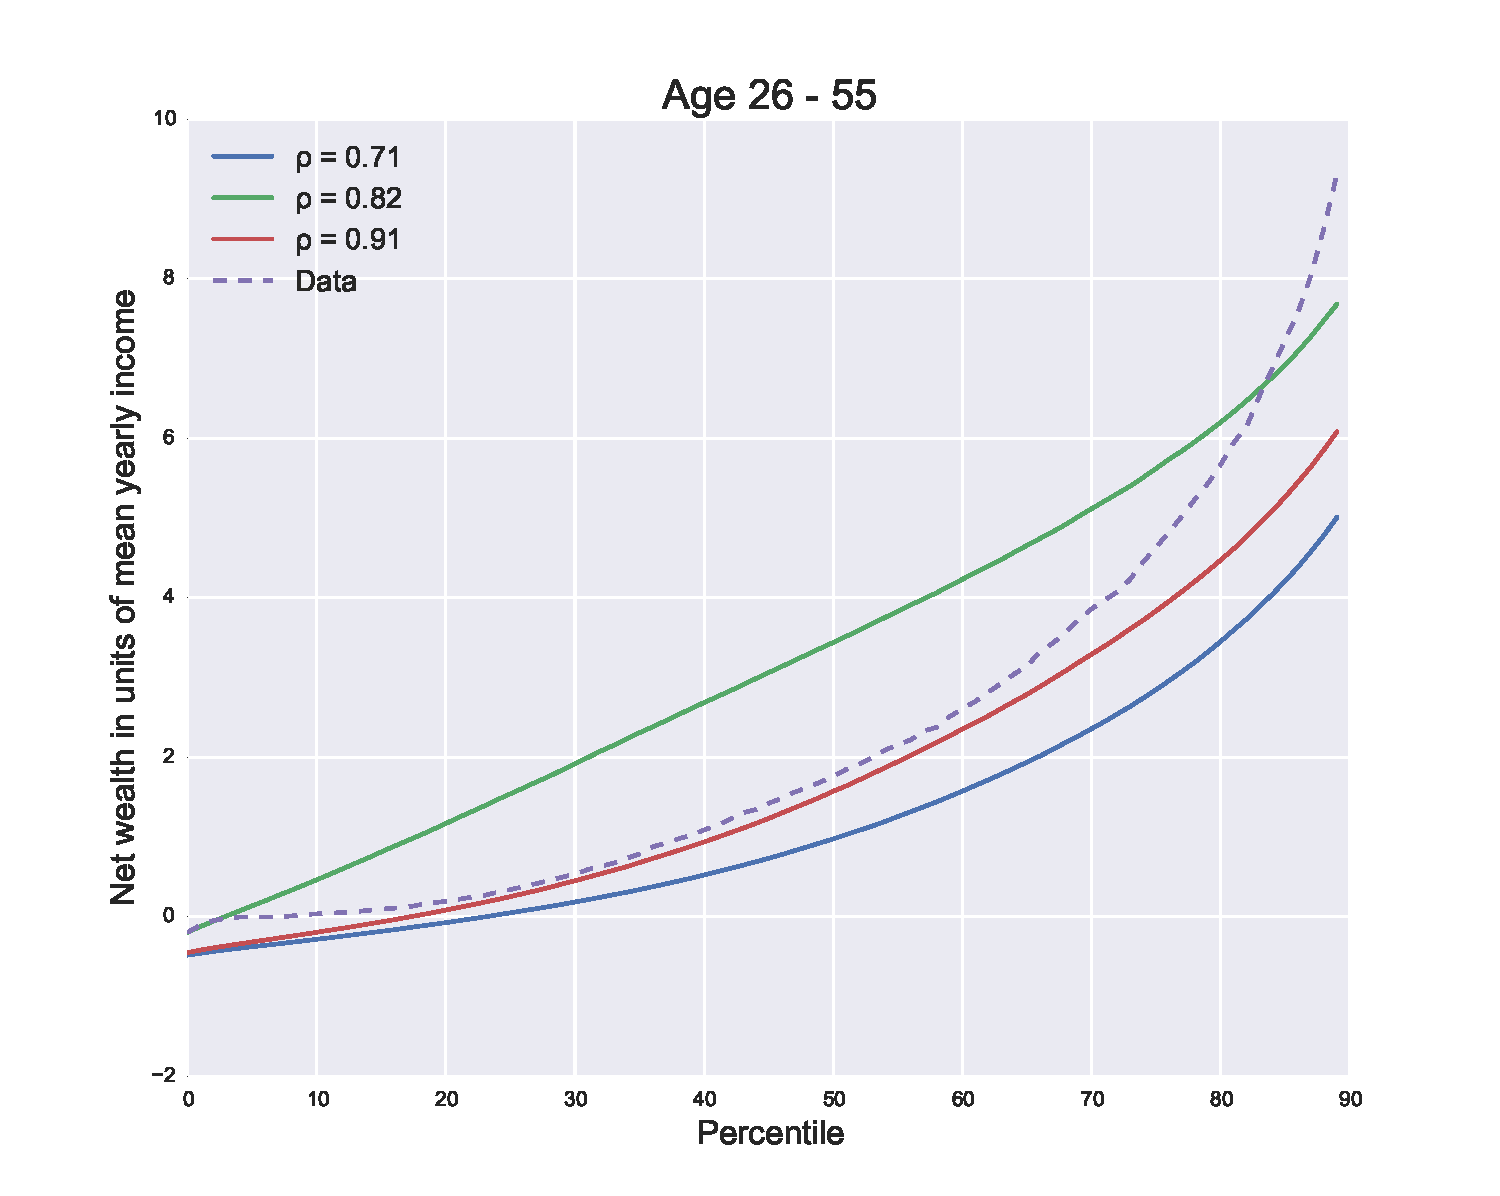
\includegraphics[width=\columnwidth]{comp_stat_rho}
\caption{Comparative statics for variance of individual-specific intercepts, prime age}
\label{fig:comp_stat_rho}
\end{figure}

\begin{figure}
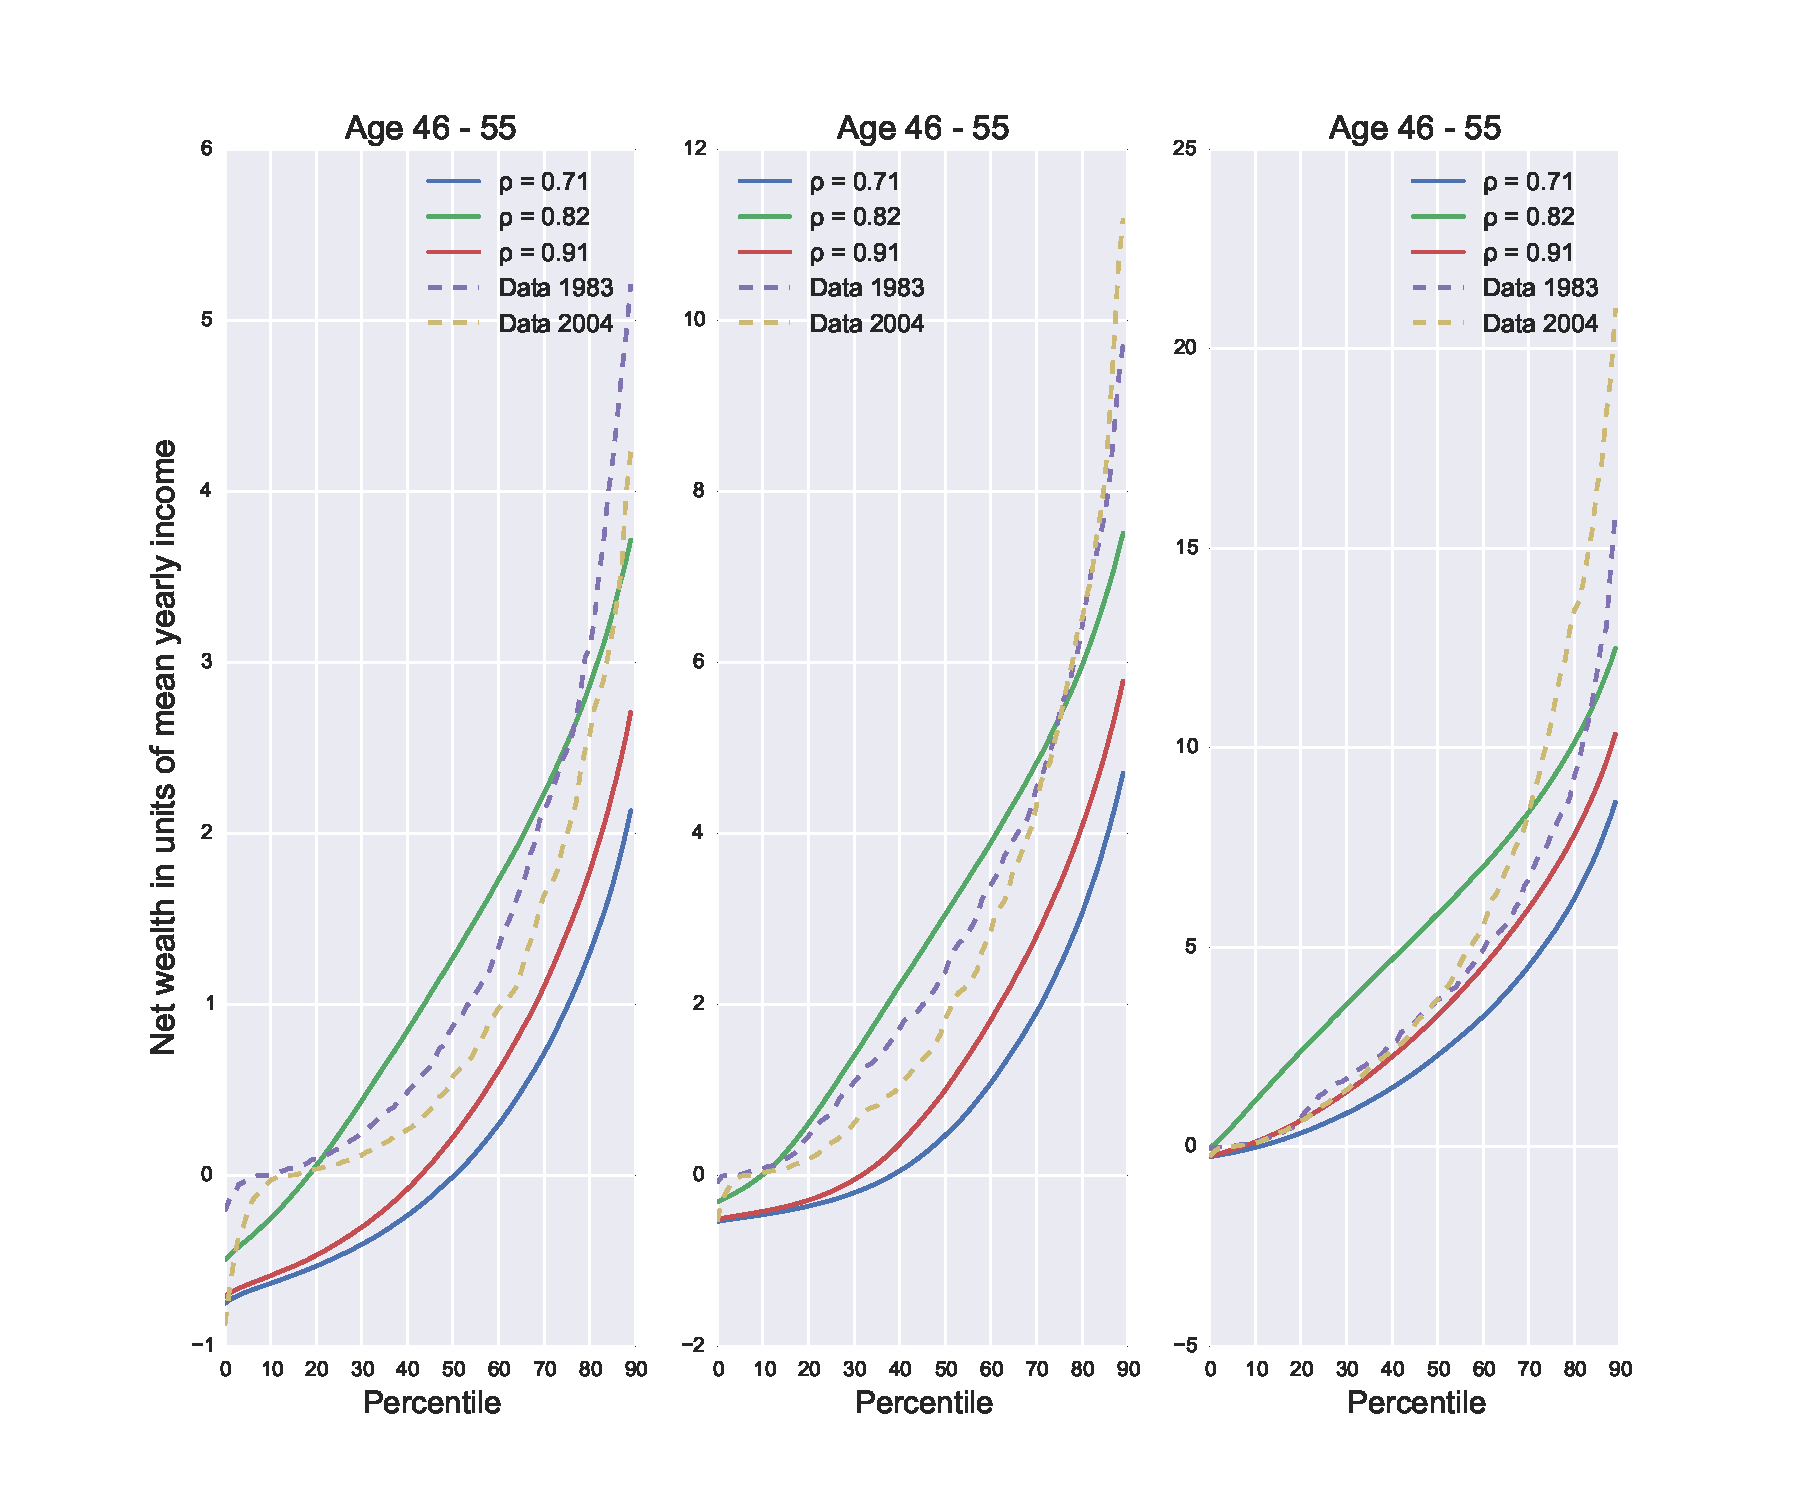
\includegraphics[width=\columnwidth]{comp_stat_rho_agedetail}
\caption{Comparative statics for variance of individual-specific intercepts, by age groups}
\label{fig:comp_stat_rho_agedetail}
\end{figure}

\begin{figure}
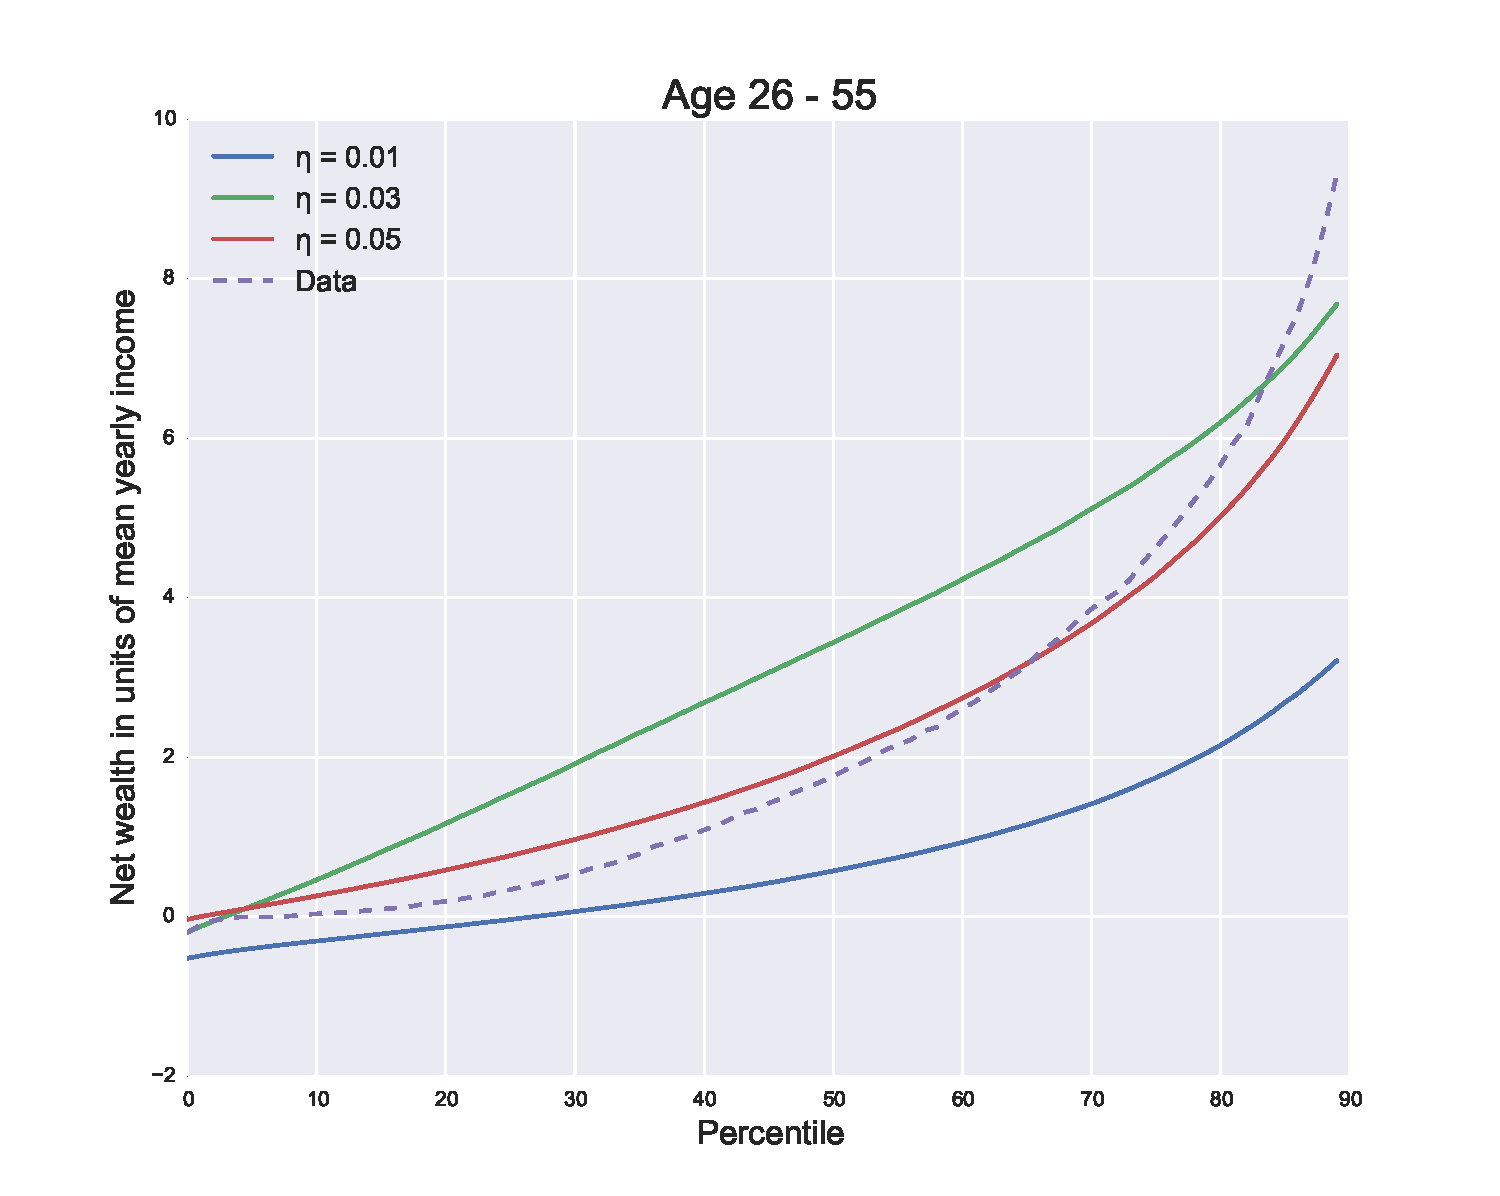
\includegraphics[width=\columnwidth]{comp_stat_eta}
\caption{Comparative statics for variance of individual-specific intercepts, prime age}
\label{fig:comp_stat_eta}
\end{figure}

\begin{figure}
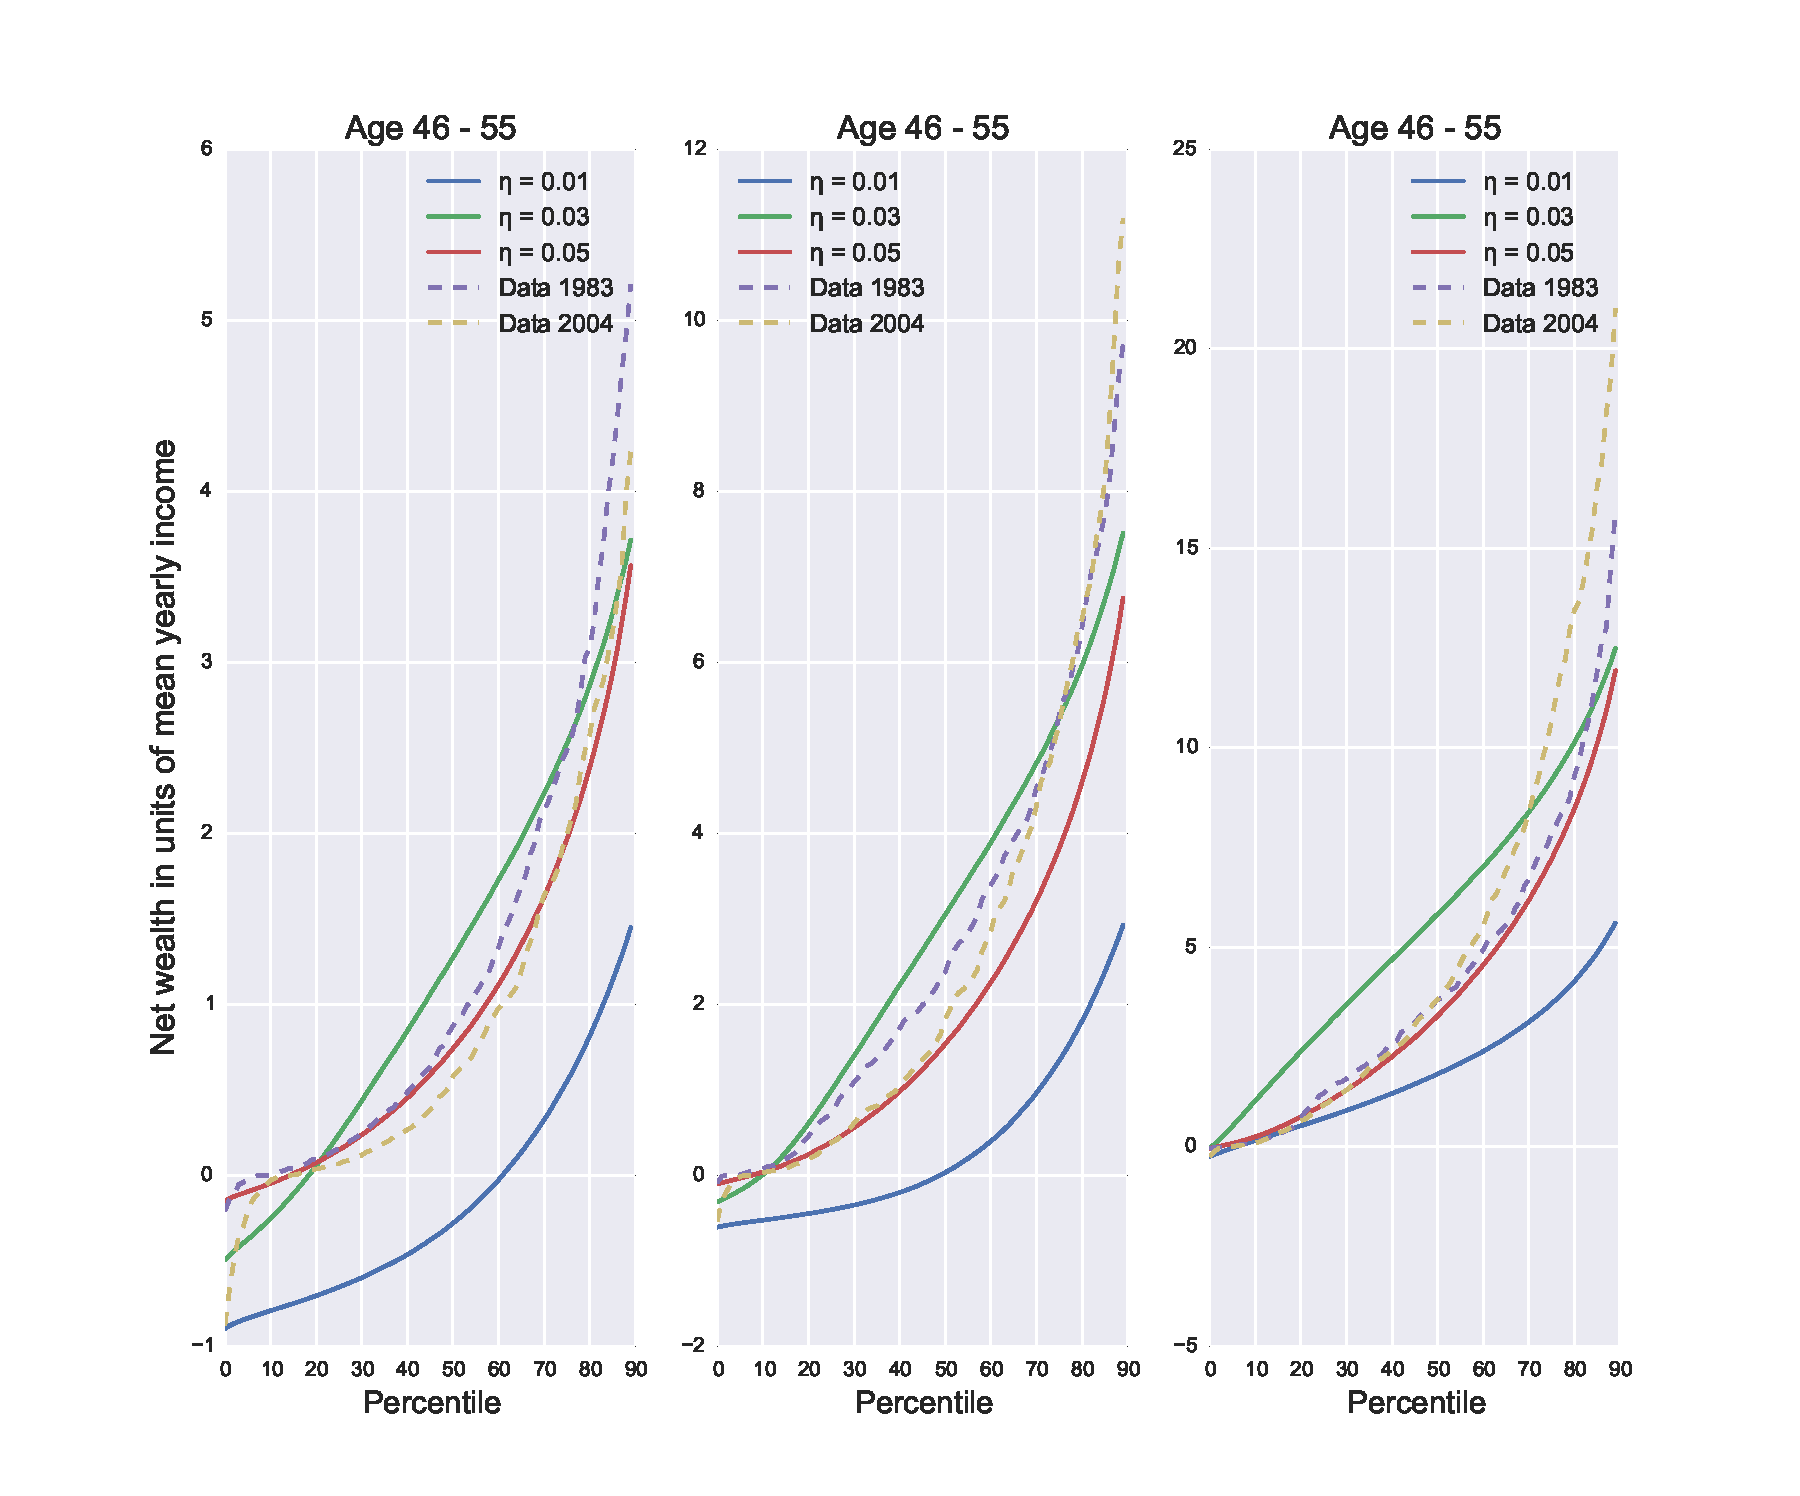
\includegraphics[width=\columnwidth]{comp_stat_eta_agedetail}
\caption{Comparative statics for variance of individual-specific intercepts, by age groups}
\label{fig:comp_stat_eta_agedetail}
\end{figure}

\begin{figure}
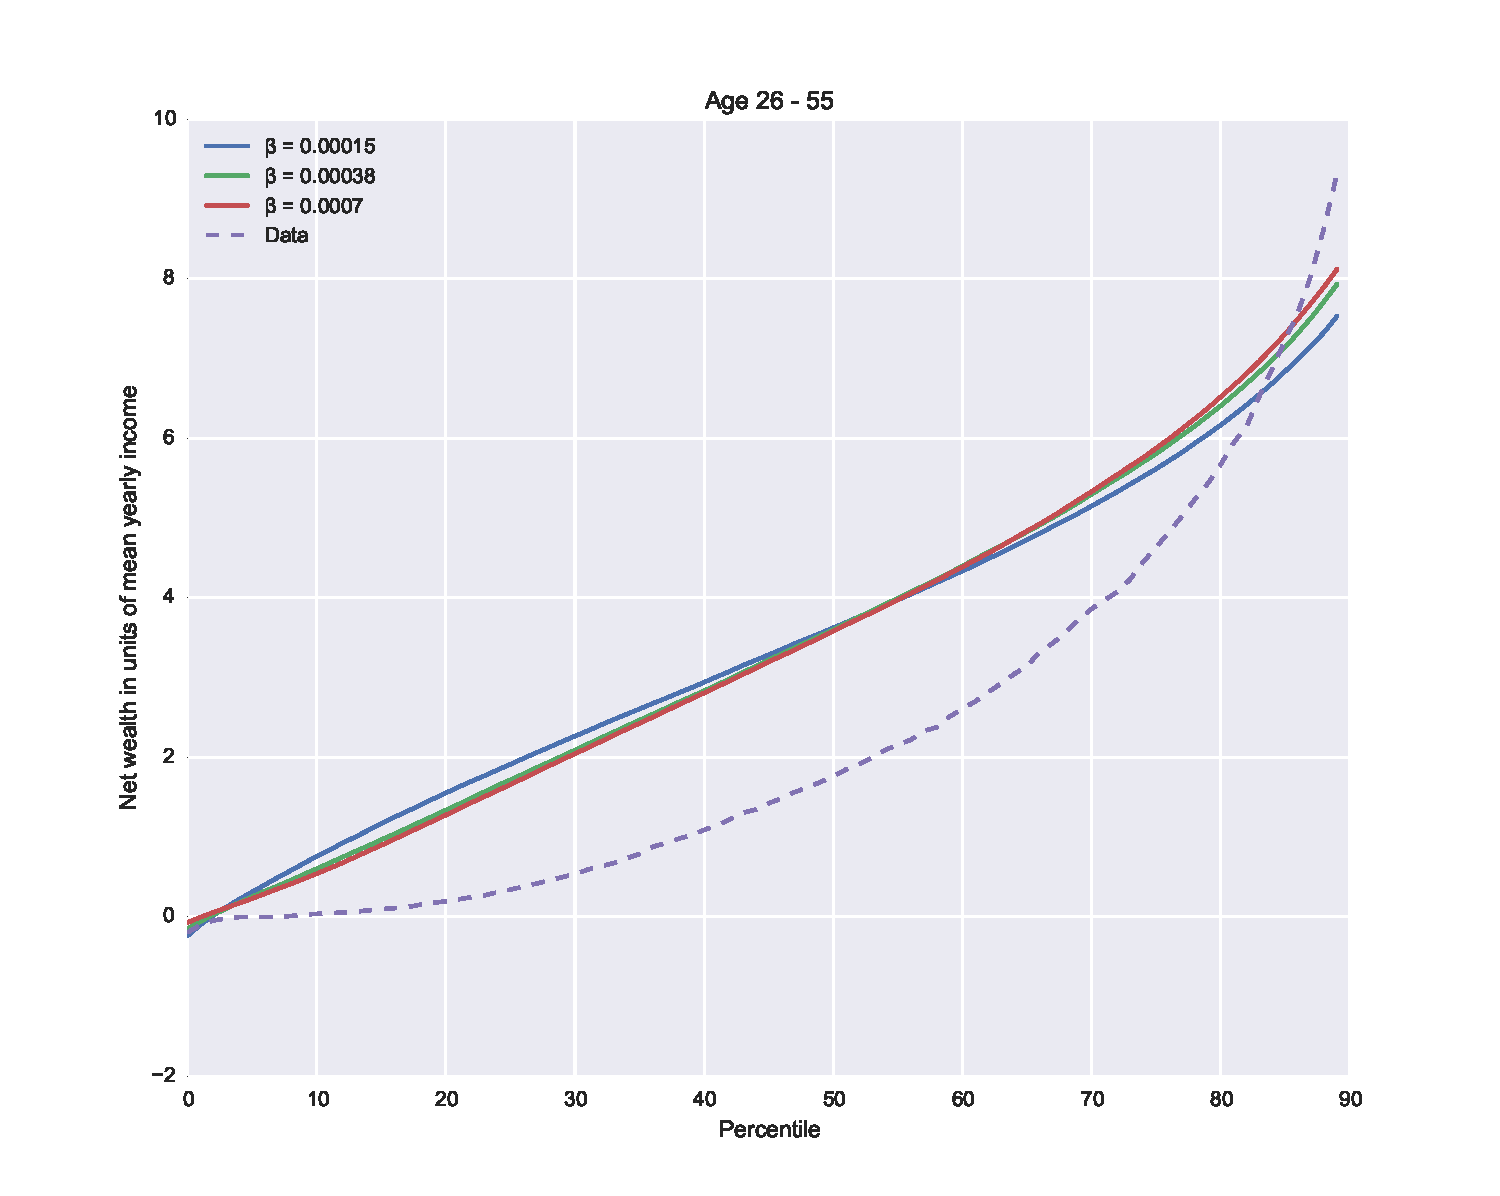
\includegraphics[width=\columnwidth]{comp_stat_beta}
\caption{Comparative statics for variance of individual-specific growth rates, prime age}
\label{fig:comp_stat_beta}
\end{figure}

\begin{figure}
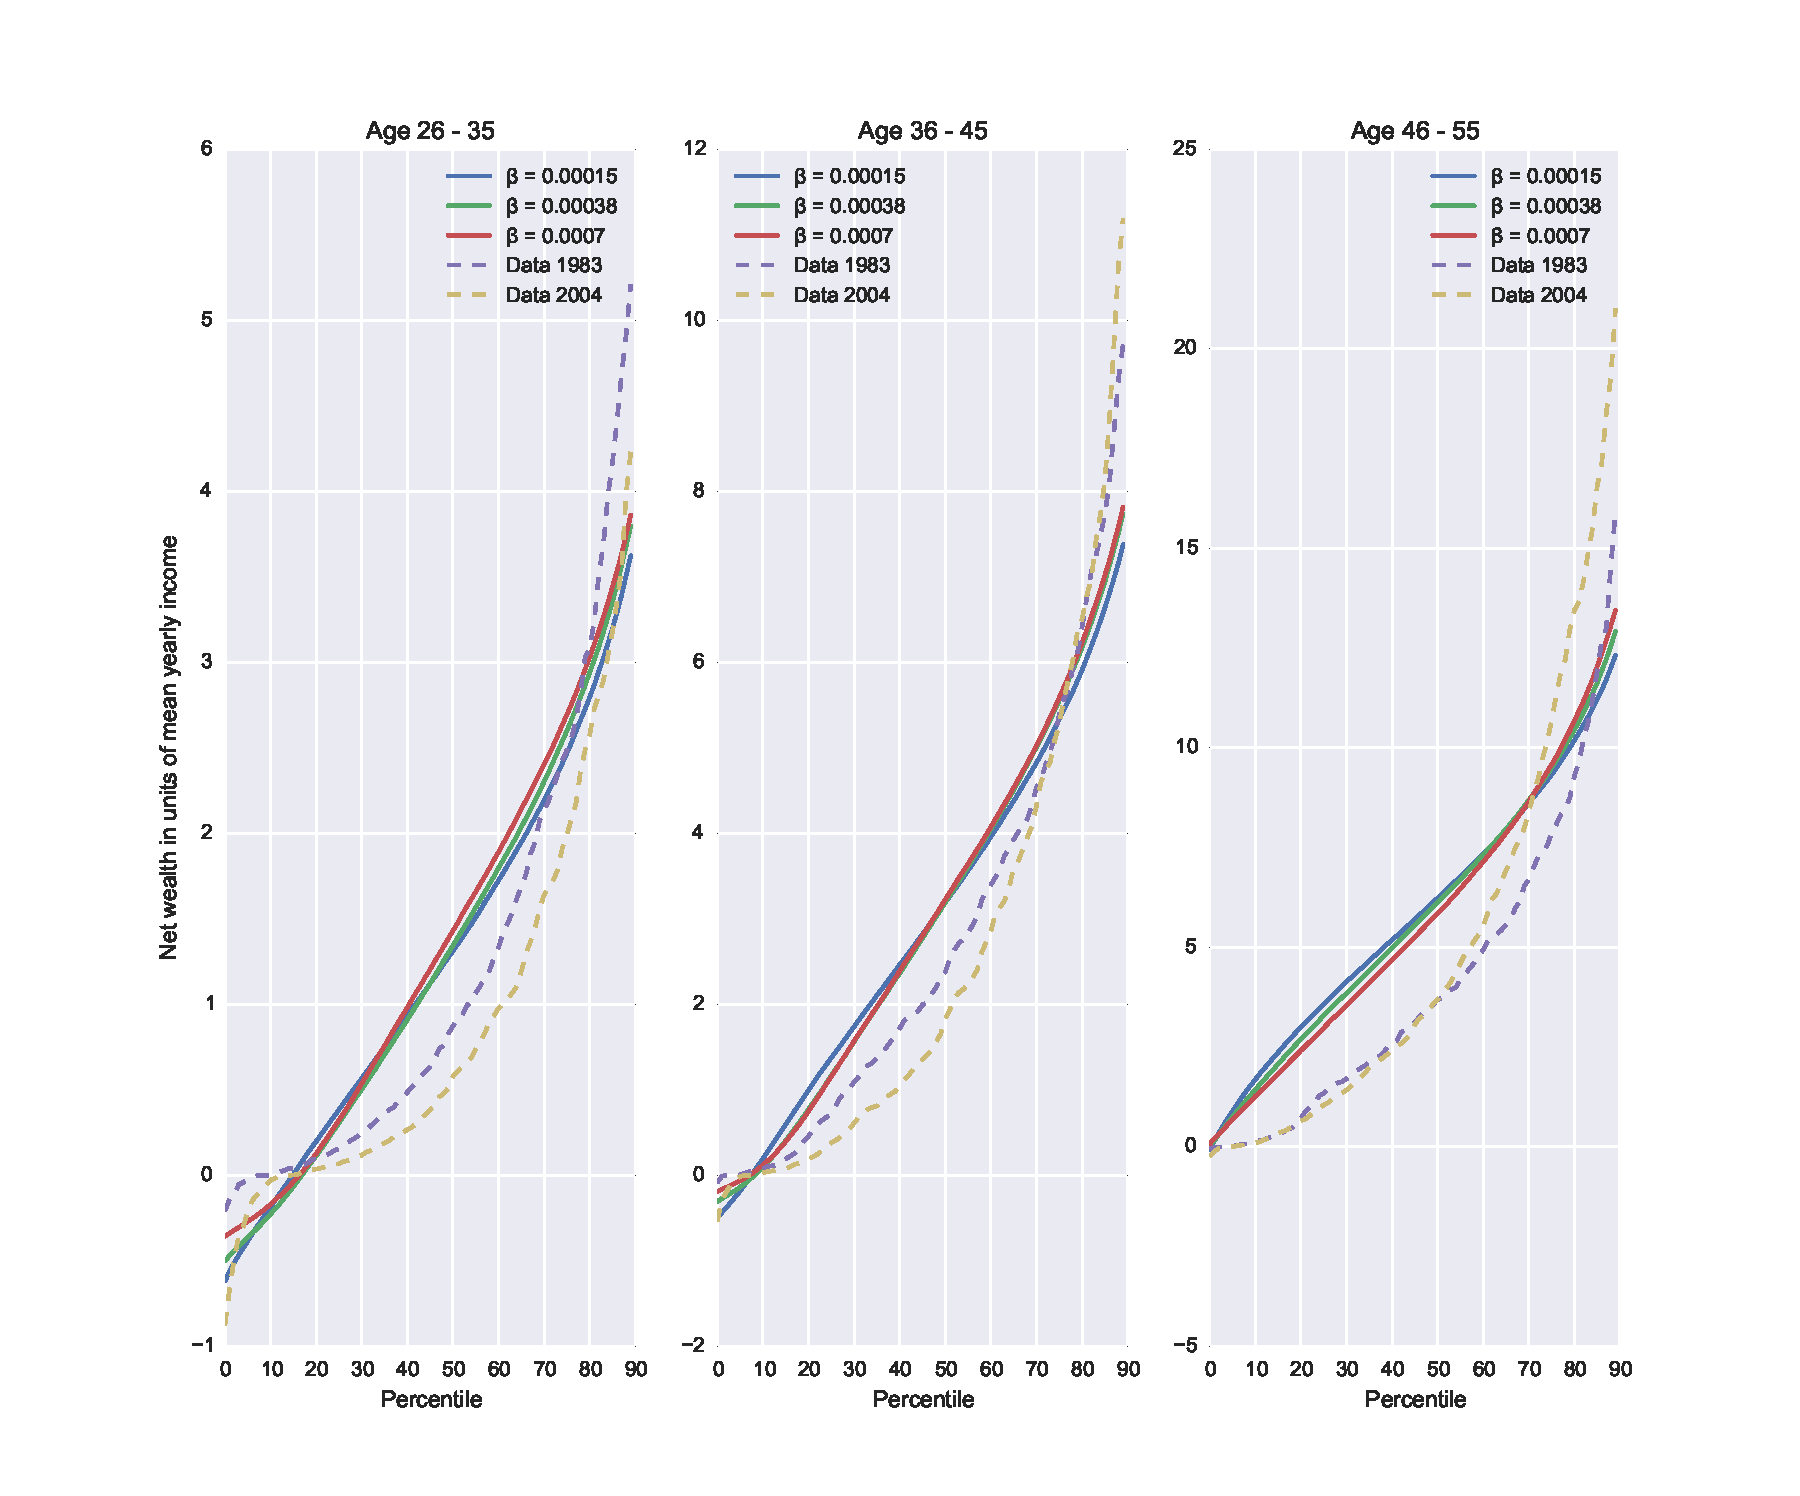
\includegraphics[width=\columnwidth]{comp_stat_beta_agedetail}
\caption{Comparative statics for variance of individual-specific growth rates, by age groups}
\label{fig:comp_stat_beta_agedetail}
\end{figure}


An important part of the mechanism explored quantitatively above was the interaction 
between profile heterogeneity, initial beliefs and learning, the speed of which 
in turn depended on the nature of the income process underlying the simulations. 
Obviously, estimating the model using a more standard income process without 
profile heterogeneity, as is done in most of the life-cycle literature, would 
eliminate this mechanism completely, as there would be no meaningful learning 
about the income process. However, recent work by \citet{Hoffmann2013} shows 
that specification error in the income process can severely bias econometric
 results towards either over- or underestimating the importance of profile 
heterogeneity. Hoffmann proposes a more general and flexible specification, 
which is still tractable enough to be used in a dynamic programming problem.

\pagebreak
\section{Discussion}\label{sec:discussion}
As this chapter has shown, the learning model of heterogeneous income processes
fails in capturing the dynamics of the wealth distribution under all calibrations
derived from empirical data on income processes. Comparing the model output of 
different counterfactual parametrisations, it became clear that the main reason
behind this is not the learning mechanism itself, but the different income 
distribution and risk implied by the heterogeneous income process. To salvage 
the model, ad-hoc changes to the belief structure of agents can be made, although
at this point it becomes a bit of a free-for-all and the model can be made to
predict any pattern in the data with a suitable choice of initial beliefs.
Building on the work in this chapter, future research should consider the implications
of other more realistic income processes on the wealth distribution, to the 
extent that they can be formulated parsimoniously enough not to increase the 
computational burden beyond reason. An example would be the work by 
\citet{MeghirPistaferri2004}, who model the conditional variance of income
shocks using an ARCH model and show analytically that the addition of individual-
specific heterogeneity in the innovation variance leads to both a larger dispersion
of savings rates and higher aggregate saving. A further case of interest would be
the specification derived by \citet{GKOS2015}, which adapts the income process
used in this chapter by adding two more AR(1) components with different innovation
variances, so that households are subject to potential shocks of different 
magnitude. As the evidence points to this process being the best description 
of the income risk households are facing in reality, the implications of this
process for the wealth distribution should be investigated further. 

\section{Appendix A: Comparative statics results}

\begin{figure}
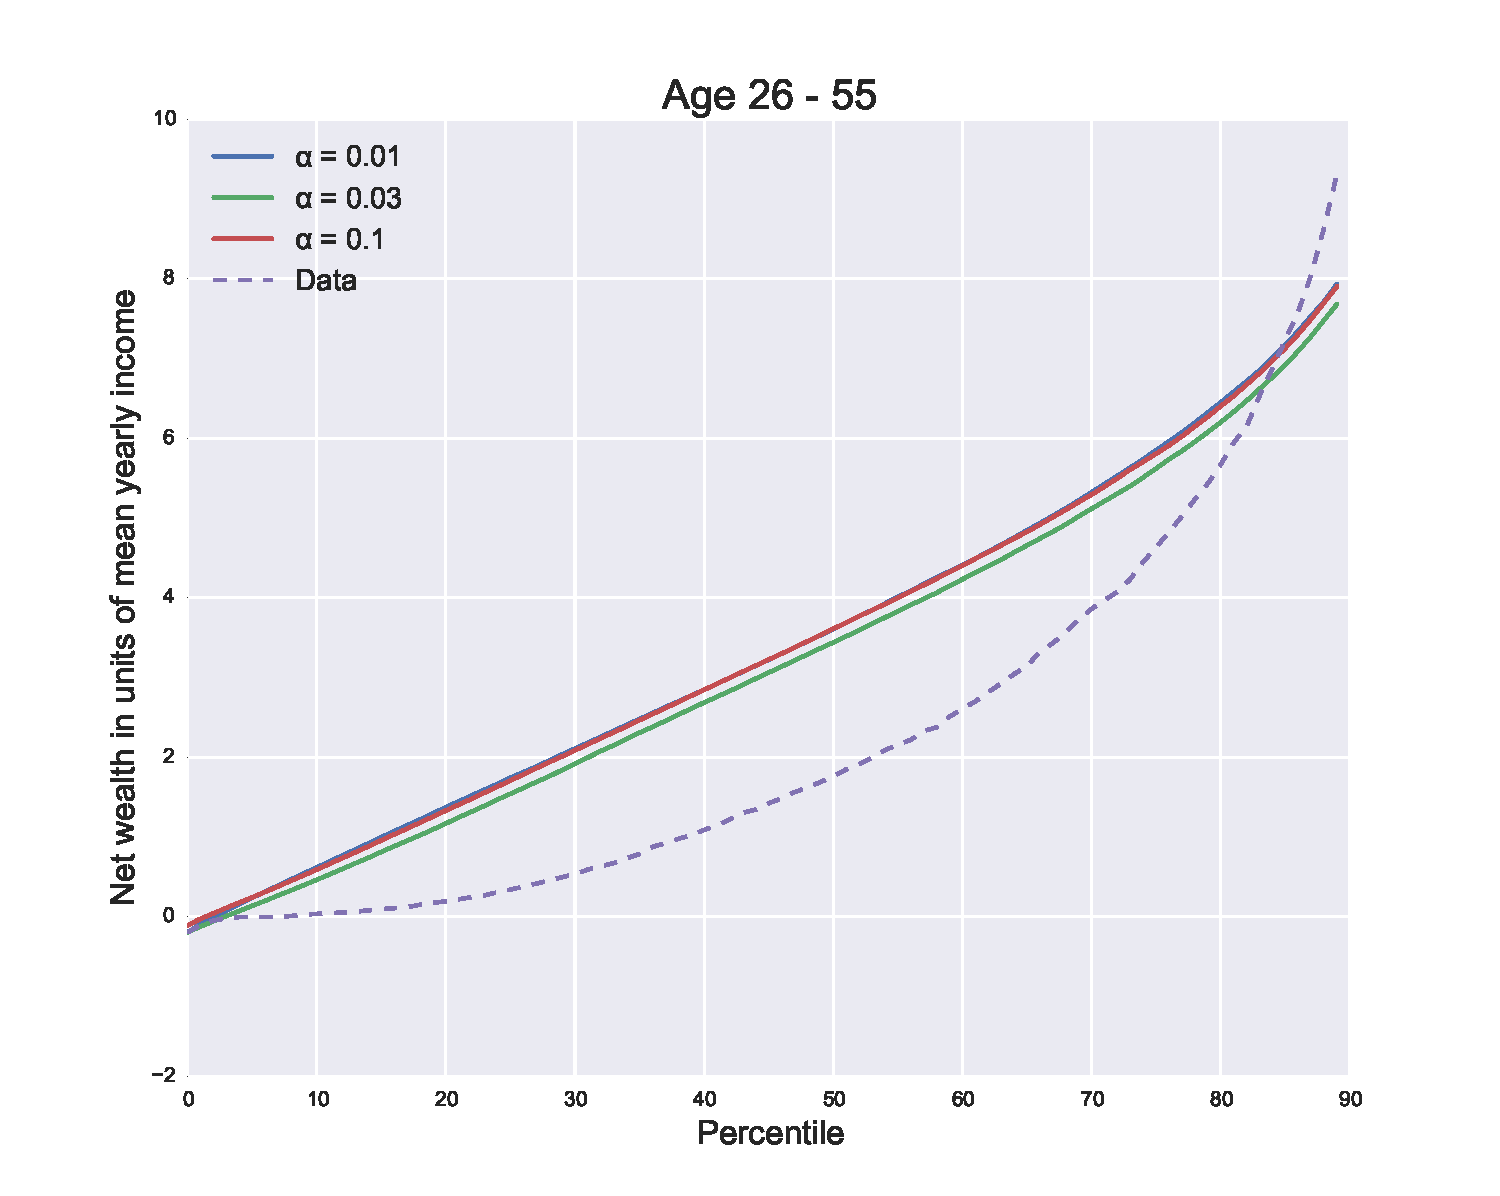
\includegraphics[width=\columnwidth]{comp_stat_alpha}
\caption{Comparative statics for variance of individual-specific intercepts, prime age}
\label{fig:comp_stat_alpha}
\end{figure}

\begin{figure}
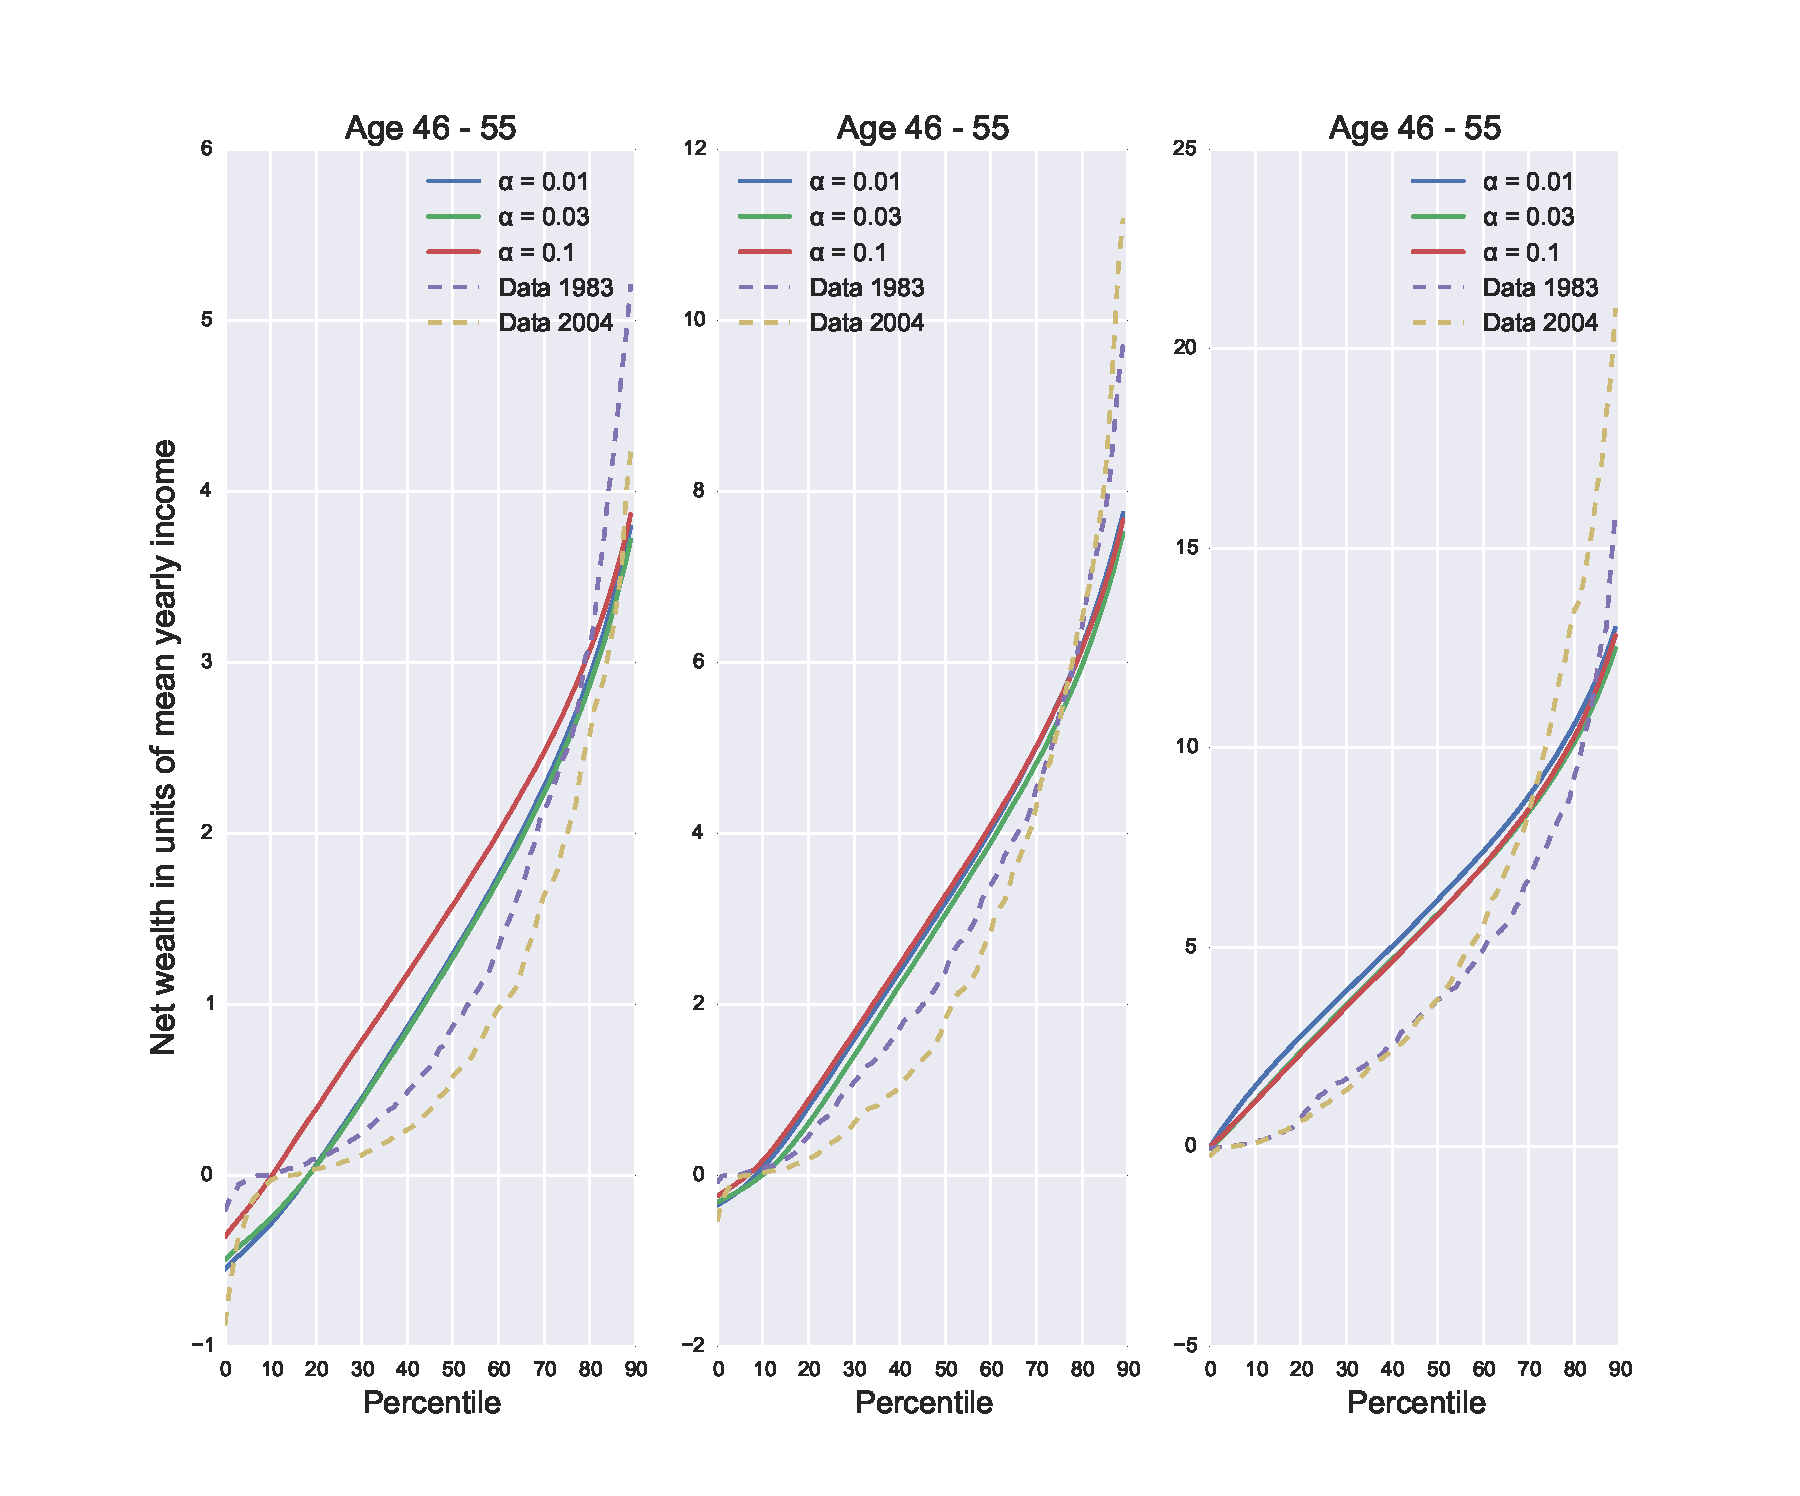
\includegraphics[width=\columnwidth]{comp_stat_alpha_agedetail}
\caption{Comparative statics for variance of individual-specific intercepts, by age group}
\label{fig:comp_stat_alpha_agedetail}
\end{figure}

\begin{figure}
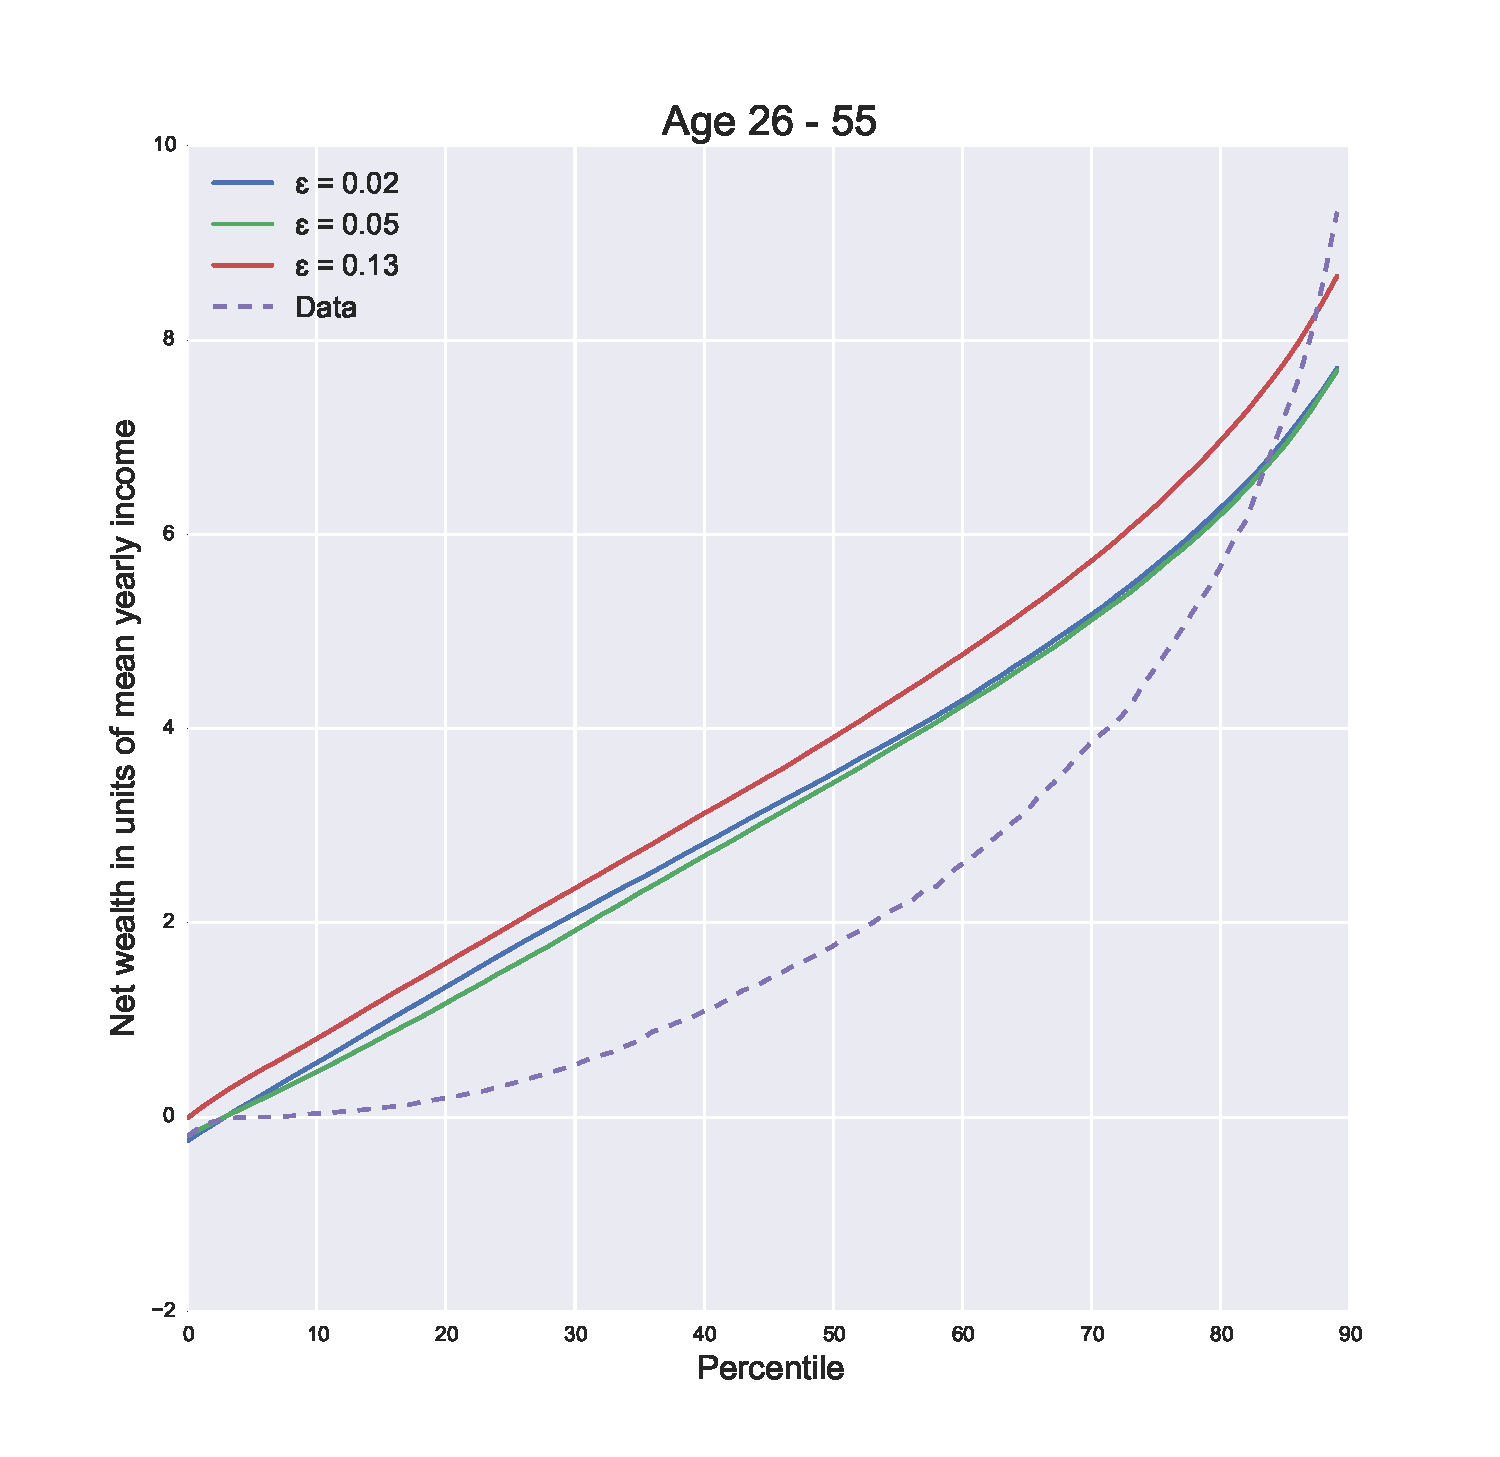
\includegraphics[width=\columnwidth]{comp_stat_eps}
\caption{Comparative statics for variance of transitory shocks, prime age}
\label{fig:comp_stat_eps}
\end{figure}

\begin{figure}
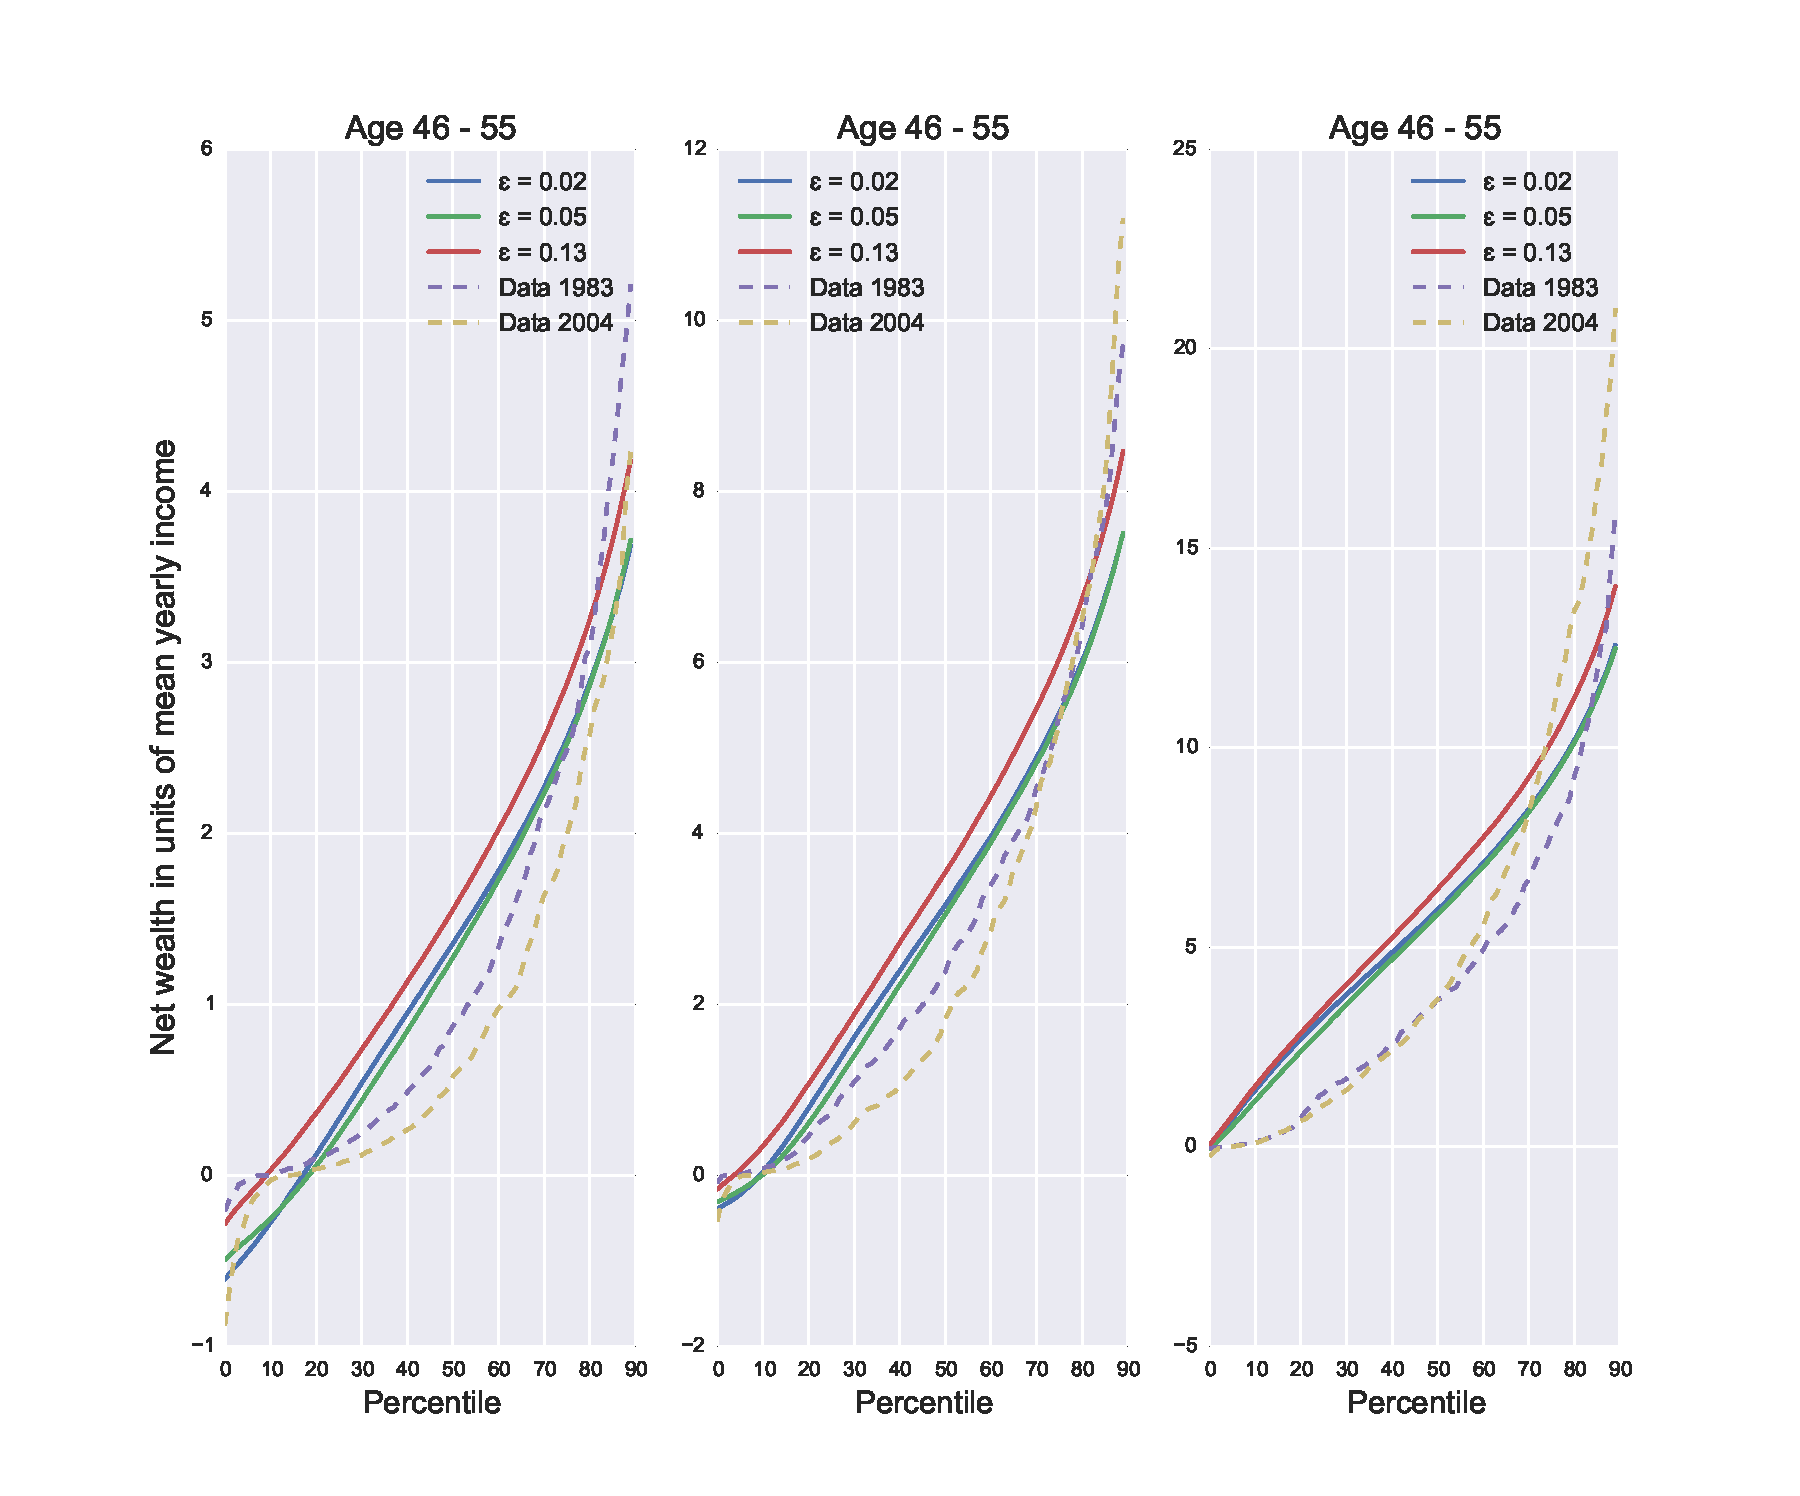
\includegraphics[width=\columnwidth]{comp_stat_eps_agedetail}
\caption{Comparative statics for variance of transitory shocks, by age group}
\label{fig:comp_stat_eps_agedetail}
\end{figure}

\begin{figure}
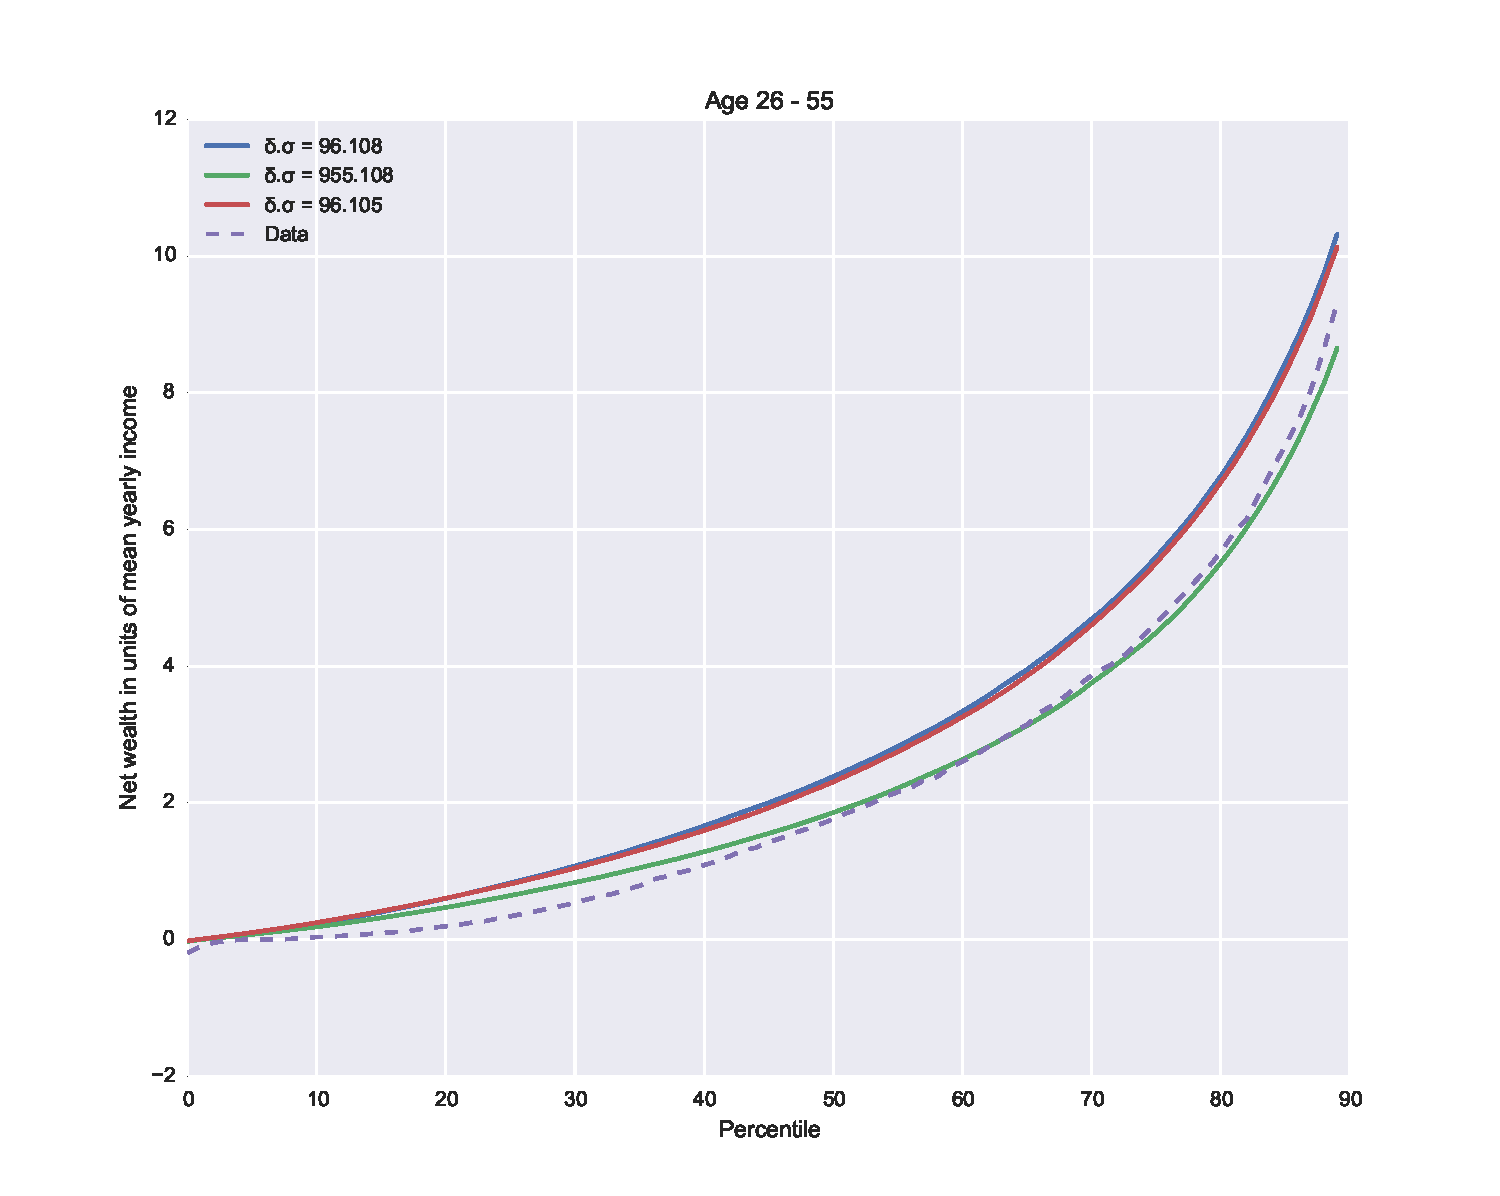
\includegraphics[width=\columnwidth]{winfriedcompare}
\caption{Model fit when income is an RIP process with $\rho=0.95$ and $\sigma^2_{\eta}=0.5$}
\label{fig:winfriedcompare}
\end{figure}

\begin{figure}
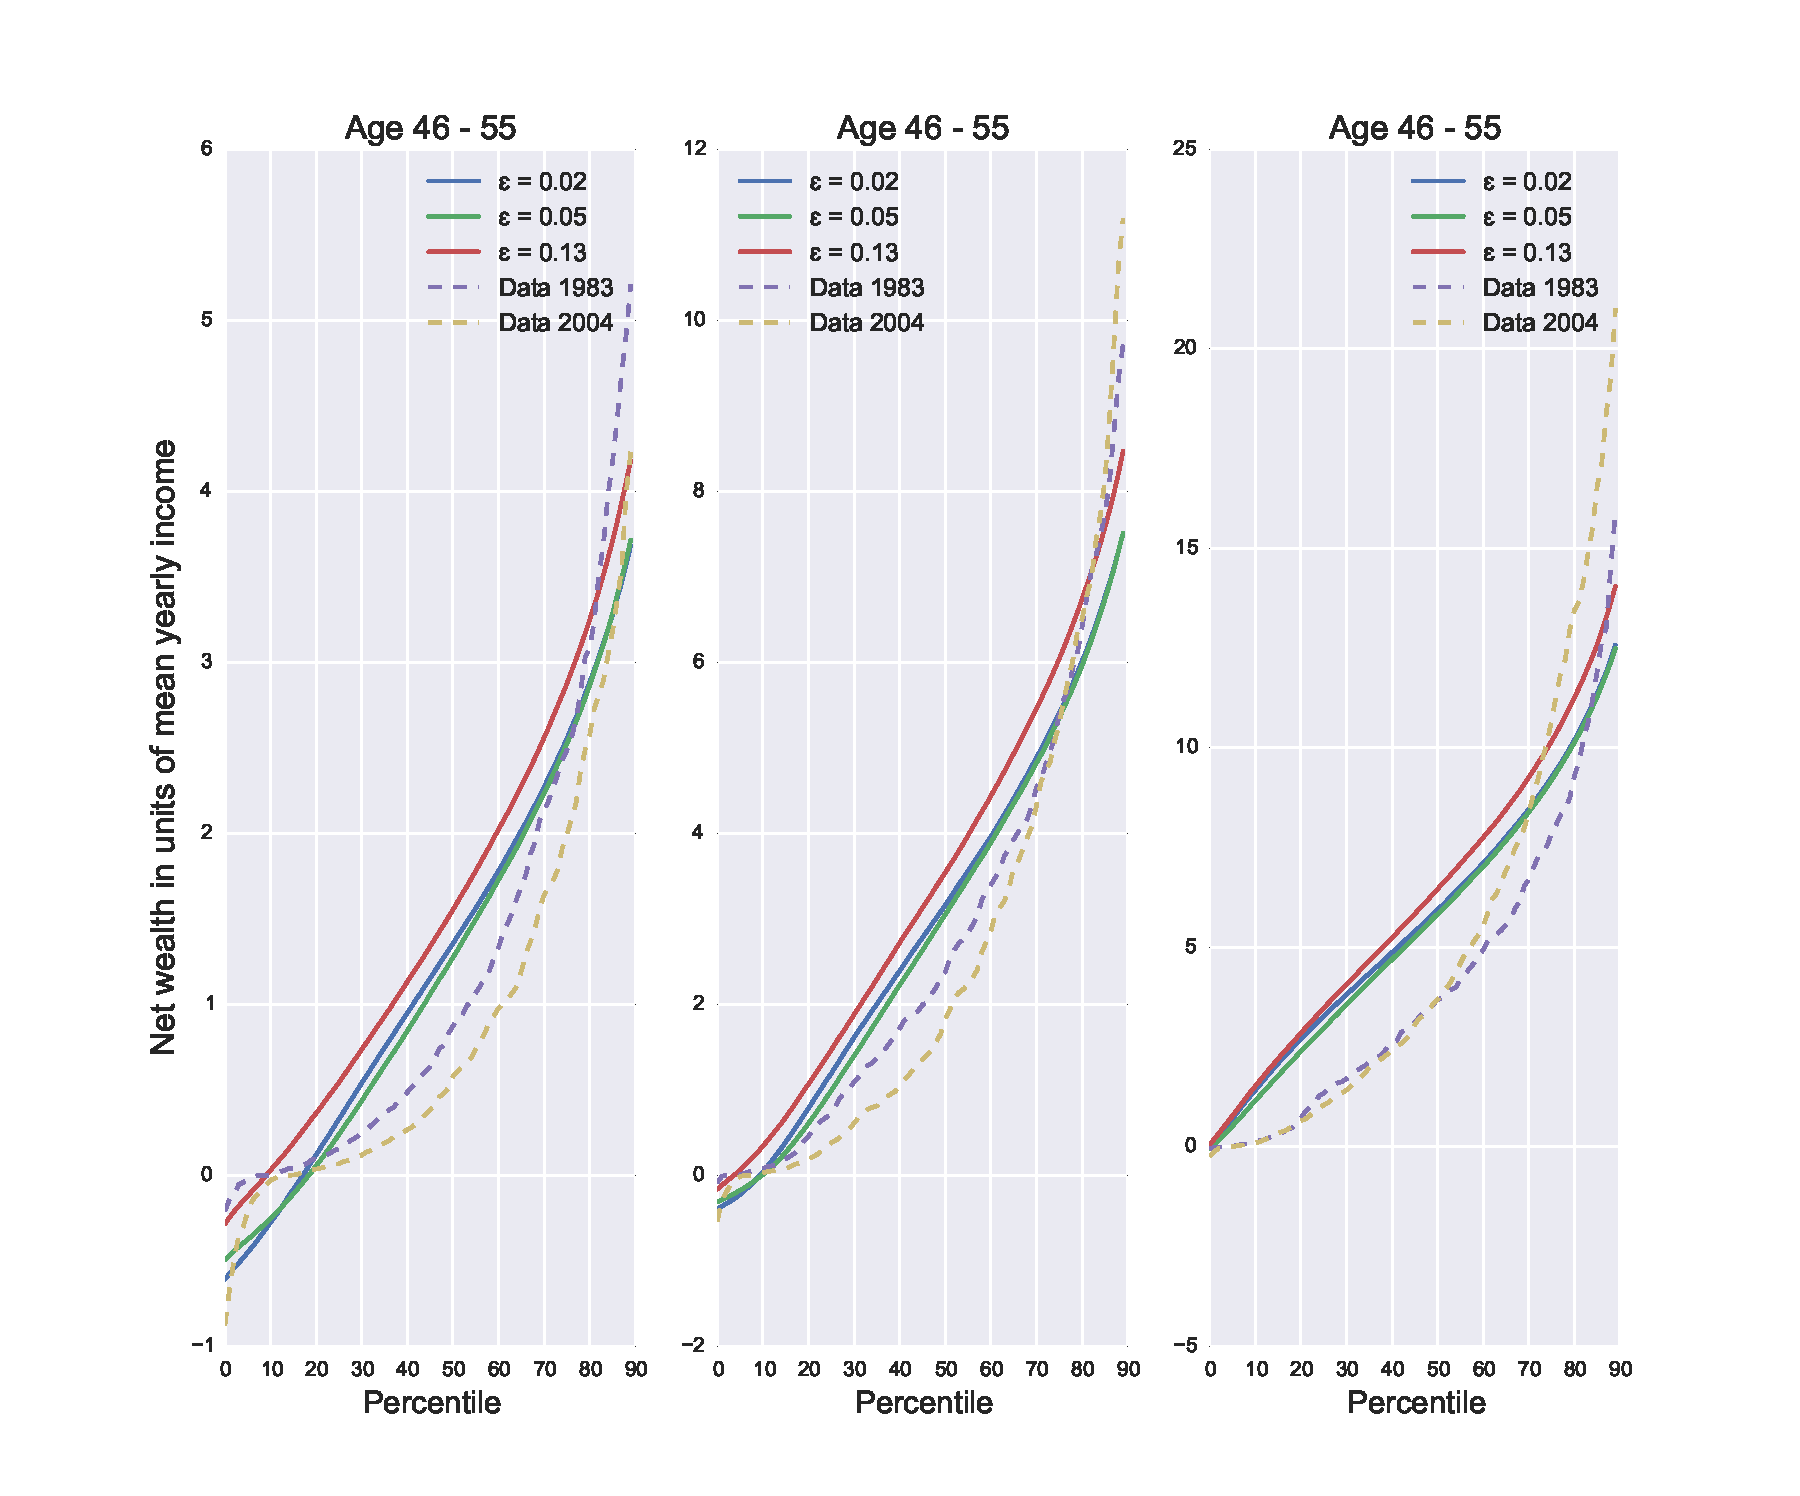
\includegraphics[width=\columnwidth]{comp_stat_eps_agedetail}
\caption{Model fit when income is an RIP process with $\rho=0.95$ and $\sigma^2_{\eta}=0.5$, by age groups}
\label{fig:winfriedcompare_agedetail}
\end{figure}

\begin{figure}
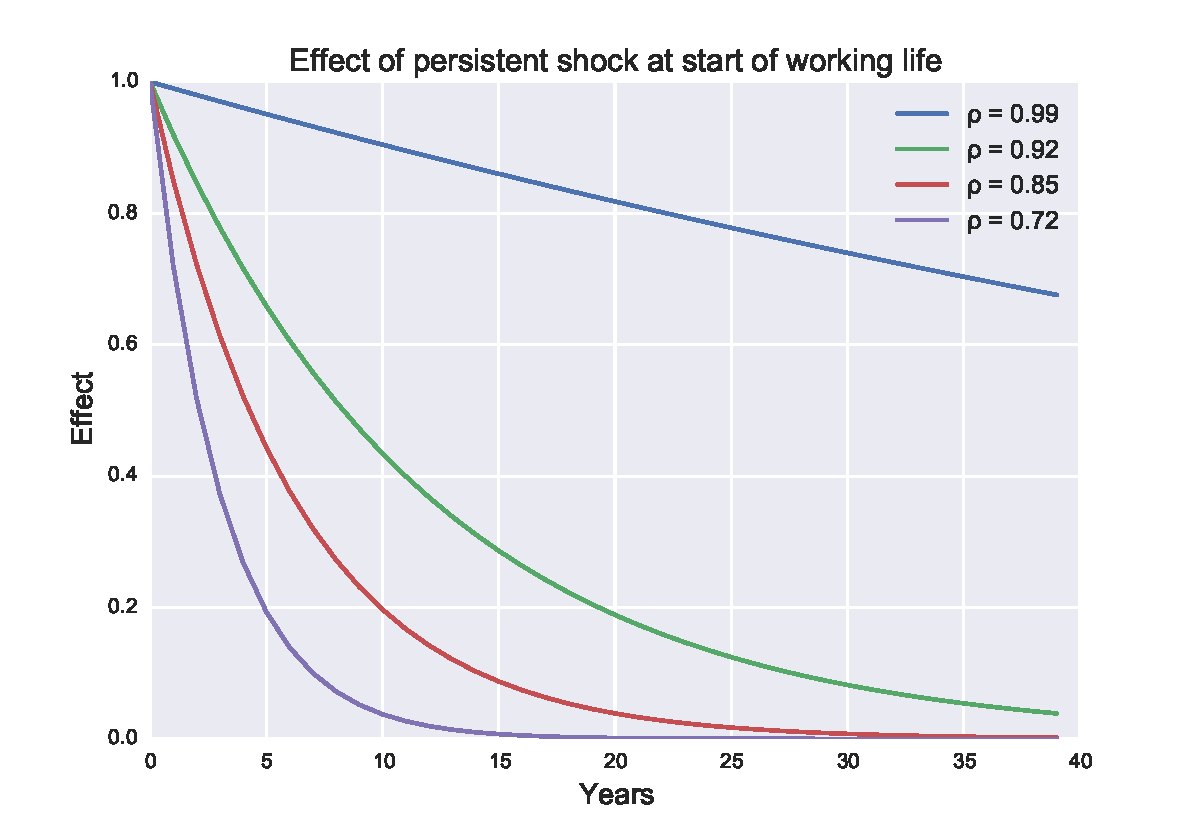
\includegraphics[width=\columnwidth]{effect_rho}
\caption{Effects of lowering $\rho$ on half life of persistent shocks}
\label{fig:effect_rho}
\end{figure}